\documentclass[conference]{IEEEtran}
\IEEEoverridecommandlockouts
% The preceding line is only needed to identify funding in the first footnote. If that is unneeded, please comment it out.
\usepackage{cite}
\usepackage{amsmath,amssymb,amsfonts}
\usepackage{algorithmic}
\usepackage{graphicx}
\usepackage{textcomp}
\usepackage{xcolor}
\usepackage{booktabs}
\usepackage{multirow}
\usepackage{url}
% \usepackage{microtype} % Disabled to prevent Overleaf free-tier 60s compilation timeouts

\def\BibTeX{{\rm B\kern-.05em{\sc i\kern-.025em b}\kern-.08em
    T\kern-.1667em\lower.7ex\hbox{E}\kern-.125emX}}

\begin{document}

\title{PVT-Invariant Parametric Fault Diagnosis in 6T SRAM Cells Using Physics-Normalized Machine Learning\\
}

\author{\IEEEauthorblockN{Shweta Gautam\IEEEauthorrefmark{1}, Archit Gupta\IEEEauthorrefmark{2}, Ayush Raj\IEEEauthorrefmark{2}, Debasish Dhungana\IEEEauthorrefmark{2}, and Vansh Singh\IEEEauthorrefmark{2}}
\IEEEauthorblockA{\IEEEauthorrefmark{1}Associate Professor, Department of Electronics and Communication Engineering, Netaji Subhas University of Technology, New Delhi, India}
\IEEEauthorblockA{\IEEEauthorrefmark{2}Department of Electronics and Communication Engineering, Netaji Subhas University of Technology, New Delhi, India}
\IEEEauthorblockA{Email: shweta.gautam@nsut.ac.in, \{archit.gupta.ug23, ayush.raj.ug23, debasish.dhungana.ug23, vansh.singh.ug23\}@nsut.ac.in}
}

\maketitle

\begin{abstract}
Embedded static random-access memory (SRAM) occupies upwards of 70\% of silicon real estate in modern system-on-chip (SoC) architectures, rendering memory yield and defect diagnosis critical to commercial semiconductor reliability. At nanoscale nodes, subtle physical defects---such as access-contact resistive opens, internal dielectric bridging, and aging-induced threshold voltage ($V_{\text{th}}$) drift---manifest as parametric degradations rather than catastrophic stuck-at faults. Consequently, classical digital March tests frequently fail to detect them. While machine learning (ML) classifiers demonstrate high diagnostic accuracy under nominal room-temperature laboratory conditions, they suffer severe out-of-distribution diagnostic collapse when deployed across broad Voltage and Temperature corners: operational environmental shifts (e.g., $>115\times$ thermal subthreshold leakage scaling and $>35\%$ gate overdrive variation) confound classifiers, dropping diagnostic accuracy on raw features from 100\% down to 46.67\%.

To overcome this fundamental challenge without requiring computationally prohibitive per-corner model retraining, this paper proposes a \textit{Physics-Informed Domain Adaptation} framework. By continuously normalizing cell metrics against a concurrent on-die reference cell ($X_{\text{inv}} = X_{\text{meas}} / X_{\text{ref}}$), common-mode environmental shifts are canceled mathematically. We validate this approach using a rigorous SPICE simulation matrix of 450 distinct instances across a 15-corner Voltage-Temperature grid (3 supply voltages $V_{DD} \in [0.9, 1.1]\,\text{V}$ $\times$ 5 temperatures $T \in \{-40, 0, 27, 75, 125\}^\circ\text{C}$) in 180\,nm CMOS, encompassing 3,150 dynamic SPICE simulations plus 105 dedicated reference characterizations. Static noise margins (SNM) are extracted using a true axis-aligned largest inscribed square algorithm on butterfly transfer characteristics. Under comprehensive Leave-One-Corner-Out (LOCO) cross-PVT evaluation across all 15 held-out corners, the proposed invariant formulation elevates Random Forest and Histogram Gradient Boosting classification accuracy from 70.67\% ($\pm 15.65\%$) and 74.00\% ($\pm 14.86\%$) (raw features) to 98.89\% ($\pm 1.63\%$) and 98.89\% ($\pm 2.05\%$), delivering a $+28.22\%$ and $+24.89\%$ generalization gain and lifting the worst-case corner accuracy floor from 46.67\% to 96.67\% and 93.33\% (with 10 of 15 corners achieving 100.0\% accuracy and exactly 5 single misclassifications across the 450-sample pooled LOCO test set). Tree SHAP explainability confirms that decision boundaries map directly to physical access impedance and dynamic switching delays.
\end{abstract}

\begin{IEEEkeywords}
6T SRAM, Parametric Faults, PVT Invariance, Machine Learning, Static Noise Margin, Domain Adaptation, Defect Diagnosis, SHAP Explainability.
\end{IEEEkeywords}

\section{Introduction}
\label{sec:intro}

The relentless scaling of complementary metal-oxide-semiconductor (CMOS) technologies into deep sub-micron nodes has propelled embedded static random-access memory (SRAM) to constitute more than 70\% to 80\% of modern System-on-Chip (SoC) dies \cite{mukhopadhyay2005modeling}. Consequently, memory yield, defect resilience, and post-silicon diagnostic fidelity represent the primary determinants of total wafer cost and field longevity in mission-critical applications spanning aerospace, automotive electronics, and ultra-low-power biomedical devices.

In nanoscale dimensions, the dominant yield-detracting mechanisms have fundamentally shifted from hard, catastrophic defects (e.g., complete open circuits or direct power-to-ground shorts) to subtle parametric imperfections \cite{marchal2008sram}. These include incomplete contact/via etch (resistive opens), thin-oxide inter-layer leakage slivers (weak bridging faults), and spatial asymmetry induced by Negative/Positive Bias Temperature Instability (NBTI/PBTI) and Hot-Carrier Injection (HCI) aging ($V_{\text{th}}$ shifts). Because these non-catastrophic faults allow cells to retain and switch logical states at nominal supply voltages and room temperature, traditional algorithmic functional patterns---such as digital March C-, March B, or Mats+ tests---routinely classify them as healthy \cite{marchal2008sram}. Nevertheless, these marginalized cells exhibit drastically compromised Static Noise Margins (SNM), latent write failures under dynamic supply fluctuations, and elevated standby leakage current ($I_{\text{DDQ}}$).

\begin{figure}[t]
\centering
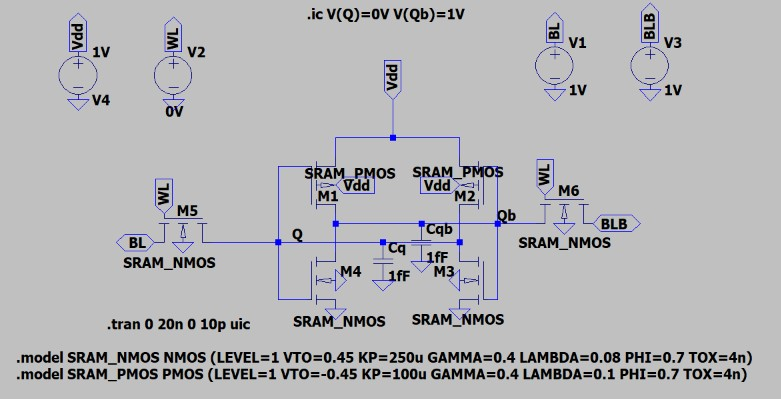
\includegraphics[width=0.95\linewidth]{6T_SRAM_LTSPICE.jpg}
\caption{Schematic of the symmetrical 180\,nm 6T SRAM cell implemented in LTspice under Hold configuration ($WL=0\,\text{V}$), showing cross-coupled inverters ($M_1$–$M_4$), access pass-gates ($M_5, M_6$), and internal storage nodes ($Q, Q_b$).}
\label{fig:cell_arch}
\end{figure}

To detect and categorize these latent flaws before catastrophic deployment failure, analog built-in current testing ($I_{\text{DDQ}}$) and machine-learning-assisted diagnosis have recently gained substantial traction. Supervised classifiers---such as Random Forests (RF), Support Vector Machines (SVM), and Gradient Boosted Decision Trees---can map high-dimensional analog signatures (timing delays, quiescent currents, bitline sense swings) into multi-class defect categories with near-perfect accuracy under nominal testing conditions ($27^\circ\text{C}, 1.0\,\text{V}$).

\textbf{The Cross-PVT Domain Shift Failure:} Despite nominal success, classical ML approaches encounter an existential operational barrier when deployed across the real-world Process, Voltage, and Temperature (PVT) operating envelope ($-40^\circ\text{C}$ to $+125^\circ\text{C}$, $\pm 10\%$ $V_{DD}$). Device physics dictates that subthreshold leakage current scales exponentially with temperature ($I_{\text{sub}} \propto T^2 \exp(-qV_{\text{th}}/kT)$), shifting nominal standby currents by over $115\times$ across the thermal envelope. Concurrently, reducing supply voltage by $10\%$ degrades transistor gate overdrive ($V_{GS} - V_{\text{th}}$), expanding dynamic write switching delay ($t_{\text{write}}$) by more than $35\%$. When an ML model trained exclusively at room temperature encounters these extreme operating corners, it misinterprets environmental physical drift as structural circuit defects. Consequently, healthy cells operating at $125^\circ\text{C}$ are erroneously flagged as internal bridging shorts, while cold healthy cells at $-40^\circ\text{C}$ and $0.9\,\text{V}$ are diagnosed as access pass-gate resistive opens. As our empirical baseline demonstrates, this out-of-distribution (OOD) domain shift drops raw classifier cross-corner accuracy to a $70.67\%$ mean with an unacceptable $46.67\%$ worst-corner floor, while traditional fixed $3\sigma$ threshold rule detectors collapse to a $3.33\%$ baseline.

To solve this without undertaking prohibitive, combinatorial training across all environmental corners, this paper introduces a \textbf{Physics-Informed Domain Adaptation} methodology. By referencing the measurements of the target cell against a concurrent, on-die reference cell simulated under the identical instantaneous PVT state ($X_{\text{inv}} = X_{\text{meas}} / X_{\text{ref}}$), we cancel common-mode environmental variance. We target this diagnostic methodology specifically at post-silicon characterization test vehicles, dedicated scribe-line test structures, and yield-learning macros equipped with analog monitor pass-gates, where high-precision parametric signatures can be directly characterized to accelerate semiconductor process debugging. The primary contributions of this paper are:
\begin{enumerate}
    \item \textbf{A Fully Automated Multi-Operation SPICE Framework:} We develop an end-to-end Python-driven simulation and netlist mutation harness that systematically injects four continuous parametric fault classes into a validated 180\,nm 6T SRAM cell and executes Hold, Write, Read, and butterfly DC sweeps across a 15-corner Voltage-Temperature grid (3 supply voltages $\times$ 5 temperatures, encompassing 3,150 total SPICE simulations plus 105 reference runs).
    \item \textbf{Exact Pure-NumPy SNM Butterfly Extraction:} We formulate a numerically robust, axis-aligned inscribed square algorithm that calculates exact Hold and Read Static Noise Margins directly from overlapping Voltage Transfer Characteristics (VTCs), eliminating the overestimation errors inherent to the widely used $45^\circ$ coordinate rotation shortcut.
    \item \textbf{Formulation of Physics-Normalized Invariant Features:} We introduce dimensionless, reference-normalized ratios that compress environmental feature dispersion (Coefficient of Variation) by up to 100.0\% on healthy cells across the 15-corner grid while preserving distinct defect separability.
    \item \textbf{Comprehensive Cross-PVT LOCO Benchmarking:} Through rigorous Leave-One-Corner-Out (LOCO) evaluation across all 15 held-out operating corners, we demonstrate that physics-normalized features boost Random Forest cross-PVT accuracy to 98.89\% and HistGradientBoosting to 98.89\%, delivering a $+28.22\%$ generalization gain over raw features.
    \item \textbf{Model Interpretability via Tree SHAP:} We provide global and class-disaggregated SHapley Additive exPlanations (SHAP) that confirm that the decision boundaries established by the classifier correspond strictly to the underlying semiconductor physics of the defect mechanisms.
\end{enumerate}

% ======================================================================

\section{Related Work \& Problem Formulation}
\label{sec:related}

\subsection{Traditional SRAM Fault Testing}
Memory testing has historically relied on algorithmic March test sequences executed via digital Built-In Self-Test (BIST) engines \cite{marchal2008sram, vandegoor1993march}. Standard algorithms (e.g., March C-, March SS) write and read deterministic bit sequences across wordlines to uncover address-decoder faults, stuck-at faults (SAF), and state-transition faults (TF) \cite{alars2005resistive, pavlov2008sram}. While highly efficient for catastrophic digital breaks, March tests exhibit near-zero coverage for latent parametric defects because intermediate voltage degradation is restored by high inverter gain prior to bitline sampling.

Dynamic fault diagnosis through $I_{\text{DDQ}}$ quiescent current monitoring was introduced to identify subthreshold leakage paths and resistive shorts \cite{mukhopadhyay2005modeling}. However, with aggressive dimensional scaling, background subthreshold leakage from millions of defect-free parallel cells obscures the localized current signature of a single defective device, drastically diminishing the defect-to-noise ratio at elevated temperatures.

\subsection{Static Noise Margin Extraction Methodologies}
The foundational standard for SRAM stability analysis was formulated by Seevinck, List, and Lohstroh \cite{seevinck1987static}. Static Noise Margin (SNM) is defined as the maximum DC noise voltage that can be tolerated by the cross-coupled inverter latch without inducing an unintended state transition. Geometrically, SNM corresponds to the side length of the largest square that can be inscribed inside the smaller of the two lobes formed by the overlapping inverter Voltage Transfer Characteristics (VTCs):
\begin{equation}
\text{SNM} = \min(L_{\text{lobe1}}, L_{\text{lobe2}})
\label{eq:snm_def}
\end{equation}
To automate this computation, many prior works applied a coordinate transformation by rotating the axes by $45^\circ$ ($u = (V_Q - V_{Qb})/\sqrt{2}$, $v = (V_Q + V_{Qb})/\sqrt{2}$) and finding the peak separation $\Delta u / \sqrt{2}$. However, on steep rail-to-rail CMOS transition slopes where $|\mathrm{d}V_o / \mathrm{d}V_i| \gg 1$, this rotated maximum coordinate separation shortcut becomes multi-valued and overestimates the actual geometric inscribed square. In this work, we implement a direct, numerical search that guarantees exact inscribed square boundaries for both symmetric and asymmetric faulty cells.

\subsection{Machine Learning in VLSI Diagnosis and Domain Shift}
Recent research has deployed machine learning classifiers to predict SRAM yield degradation and diagnose parametric faults \cite{stratigopoulos2014ml, dasilva2018post, pedregosa2011scikit}. Typical workflows train neural networks or support vector machines on features such as write delay, bitline discharge rate, and supply currents. 

However, a fundamental flaw across existing literature is the \textit{static nominal assumption}: models are trained and tested on samples partitioned randomly from an identical nominal environment ($27^\circ\text{C}, 1.0\,\text{V}$) \cite{singh2009variability}. Under real-world deployment, variations in ambient temperature ($-40^\circ\text{C}$ to $125^\circ\text{C}$) and battery or regulator droop ($0.9\,\text{V}$ to $1.1\,\text{V}$) induce severe domain shift. Because the ML decision boundaries are trained on raw absolute magnitudes, the environmental drift mimics defect signatures, causing severe out-of-distribution diagnostic collapse. This paper specifically addresses and resolves this cross-PVT domain generalization problem.

% ======================================================================

\section{6T SRAM Circuit Architecture \& Physical Operations}
\label{sec:circuit}

\subsection{Transistor Sizing and Symmetrical Topology}
The circuit under investigation is a symmetrical 6T SRAM cell implemented in a standard 180\,nm CMOS technology node ($V_{DD,\text{nom}} = 1.0\,\text{V}$). The cell schematic is illustrated in Fig.~\ref{fig:cell_arch}, comprising two cross-coupled CMOS inverters ($M_1/M_3$ and $M_2/M_4$) and two NMOS access pass-gates ($M_5, M_6$) gated by the Wordline ($WL$). Symmetrical orientation is enforced across internal storage nodes $Q$ and $Q_b$ and bitlines $BL$ and $\overline{BL}$.

Device channel dimensions are sized against established memory stability criteria:
\begin{itemize}
    \item \textbf{Pull-down Driver NMOS ($M_3, M_4$):} $W_D = 720\,\text{nm}, L_D = 180\,\text{nm} \implies (W/L)_D = 4.0$.
    \item \textbf{Access Pass-gate NMOS ($M_5, M_6$):} $W_{AX} = 540\,\text{nm}, L_{AX} = 180\,\text{nm} \implies (W/L)_{AX} = 3.0$.
    \item \textbf{Pull-up PMOS ($M_1, M_2$):} $W_L = 360\,\text{nm}, L_L = 180\,\text{nm} \implies (W/L)_L = 2.0$.
\end{itemize}

\textbf{Stability Design Criteria:}
\begin{enumerate}
    \item \textbf{Cell Ratio ($\beta$ or CR):} To ensure read stability, the driver must overpower the access device:
    \begin{equation}
    \beta = \frac{(W/L)_{\text{driver}}}{(W/L)_{\text{access}}} = \frac{720\,\text{nm}}{540\,\text{nm}} = 1.333 > 1.2
    \end{equation}
    \item \textbf{Pull-up Ratio ($\gamma$ or PR):} To ensure writeability, the pull-up ratio must satisfy:
    \begin{equation}
    \gamma = \frac{(W/L)_{\text{pullup}}}{(W/L)_{\text{access}}} = \frac{360\,\text{nm}}{540\,\text{nm}} = 0.667 < 1.0
    \end{equation}
    (Equivalently, Writability Ratio $\mu = 1/\gamma = 1.50 > 1.0$).
\end{enumerate}

\subsection{Operational Baselines at Nominal Corner ($27^\circ\text{C}, 1.0\,\text{V}$)}
Three distinct dynamic operations and two static DC characterizations are performed:
\begin{enumerate}
    \item \textbf{Hold Mode ($WL=0\,\text{V}, BL=\overline{BL}=V_{DD}$):} Latched state retains internal nodes: $V(Q) = 1.000\,\text{V}$, $V(Q_b) = 0.000\,\text{V}$. Standby quiescent leakage current is verified at $I_{\text{DDQ}} = 14.0\,\text{nA}$.
    \item \textbf{Read 1 / Read 0 Mode:} Bitlines are precharged to $V_{DD}$ ($C_{\text{BL}} = 20\,\text{fF}$). $WL$ is stepped to $V_{DD}$. During Read 1, $Q=1$ holds $M_3$ off, while $Q_b=0$ causes $M_4$ and $M_6$ to sink bitline current, generating a differential bitline discharge $\Delta V_{\text{BL}} = 235.4\,\text{mV}$ within $t_{\text{sense}} = 64.5\,\text{ps}$. Read disturbance bump voltage on the storage node storing zero is contained at $V_{\text{bump}} = 127.9\,\text{mV} \ll V_{DD}/2$.
    \item \textbf{Write 1 / Write 0 Mode:} Driven with differential bitlines ($BL=V_{DD}, \overline{BL}=0\,\text{V}$). Wordline assertion turns on $M_6$, pulling $Q_b$ down through $0.5 V_{DD}$, regenerating the cross-coupled inverter latch. Write flip delay is measured as $t_{\text{write}} = 62.2\,\text{ps}$.
\end{enumerate}

\begin{figure}[t]
\centering
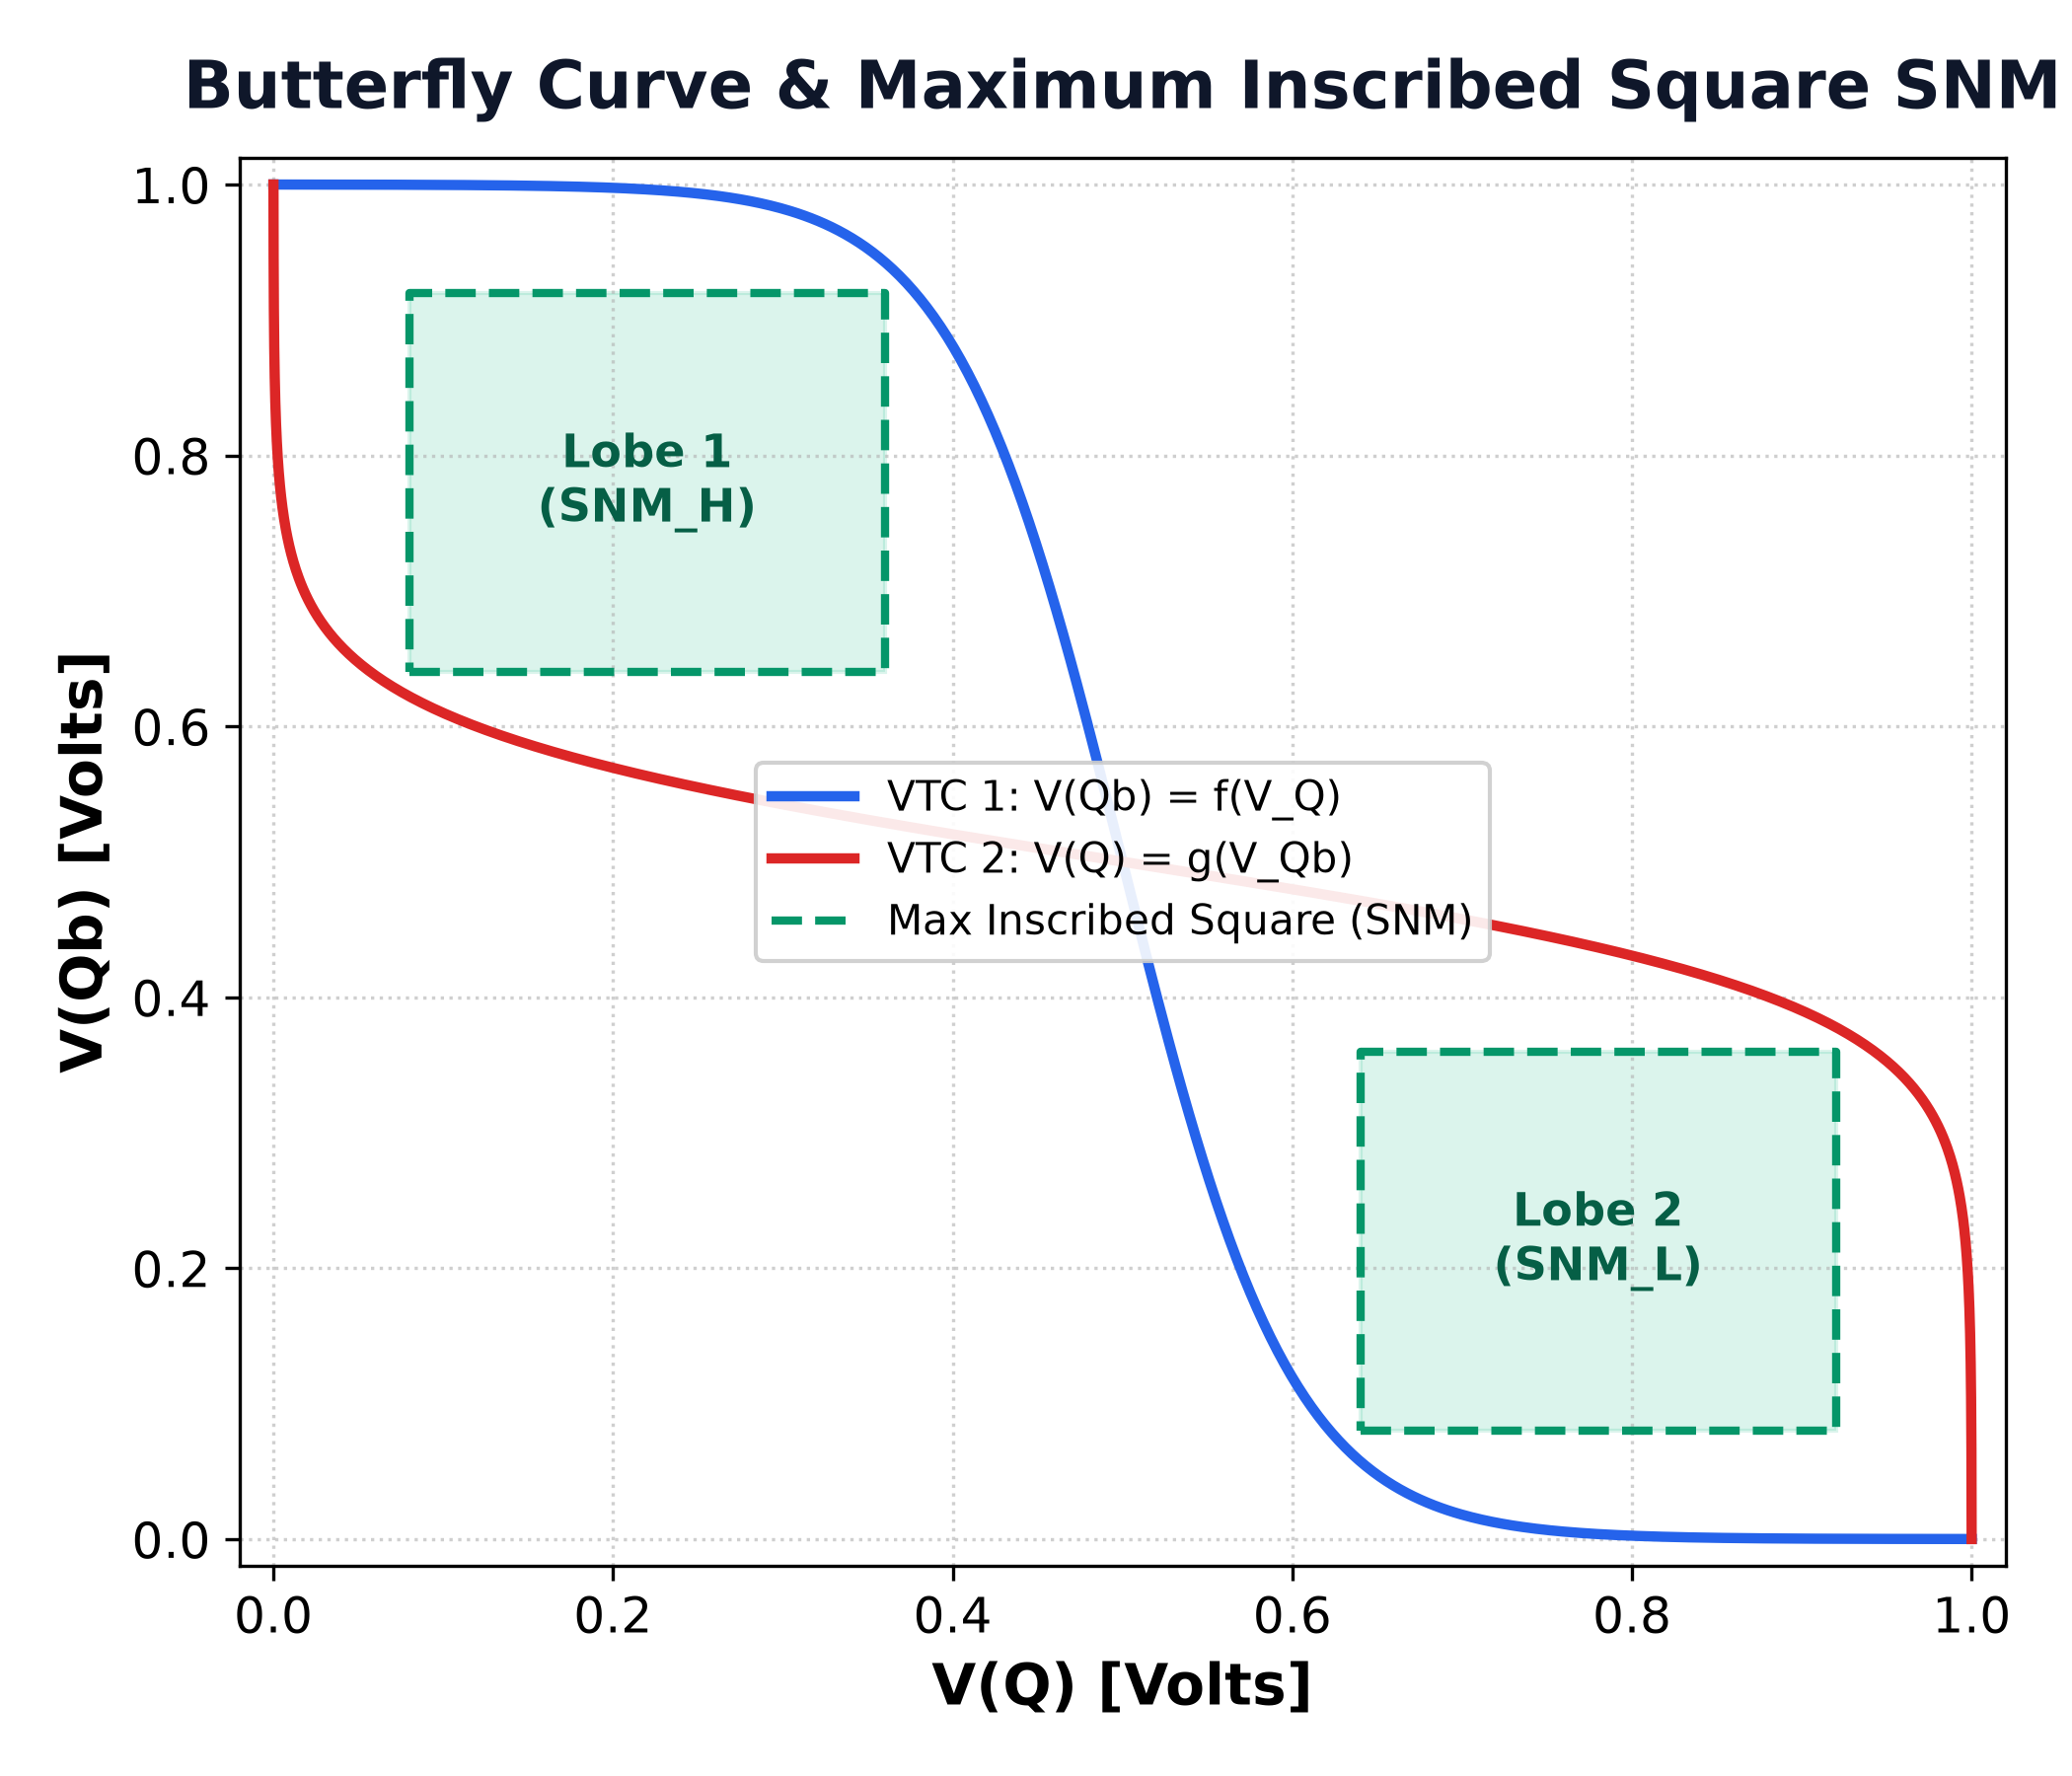
\includegraphics[width=0.92\linewidth]{snm_butterfly_diagram.png}
\caption{Voltage Transfer Characteristics (VTC butterfly curve) of the healthy 180\,nm 6T SRAM cell under Hold and Read modes, illustrating the exact inscribed squares extracted by our pure-NumPy algorithm.}
\label{fig:butterfly}
\end{figure}

\subsection{Exact Inscribed Square SNM Butterfly Extraction}
To measure Static Noise Margin, we compose dedicated DC testbenches (\texttt{stimulus\_snm\_hold.net} and \texttt{stimulus\_snm\_read.net}). The cross-coupled loop is opened in SPICE by defining a duplicated cell core (\texttt{\_c2}). A DC voltage sweep $V_5$ is applied from $0\,\text{V}$ to $V_{DD}$ in $1.0\,\text{mV}$ increments to trace $V(Q_b) = f(V_Q)$ and $V(Q) = g(V_{Q_b})$.

Our extraction engine in \texttt{src/snm\_extraction.py} finds the maximum inscribed square by solving:
\begin{equation}
\max \, s \quad \text{s.t.} \quad \forall v \in [u, u+s], \; f(v) \ge g^{-1}(v) + s \quad (\text{or dual})
\end{equation}
As reported in Table~\ref{tab:snm_val}, the automated extraction script matches golden manual measurements to within $0.06\,\text{mV}$, satisfying our strict validation criteria ($\Delta < 1.0\,\text{mV}$).

\begin{table}[t]
\centering
\caption{SNM Extraction Validation Against Golden Baselines}
\label{tab:snm_val}
\resizebox{\columnwidth}{!}{
\begin{tabular}{lcccc}
\toprule
\textbf{Operating Mode} & \textbf{Lobe 1 [mV]} & \textbf{Lobe 2 [mV]} & \textbf{SNM [mV]} & \textbf{Error vs Golden} \\
\midrule
\textbf{Hold Mode} & 470.06 & 470.06 & \textbf{470.06} & $+0.06\,\text{mV}$ \\
\textbf{Read Mode} & 263.69 & 263.69 & \textbf{263.69} & $-0.01\,\text{mV}$ \\
\bottomrule
\end{tabular}
}
\end{table}

% ======================================================================

\section{Parametric Fault Taxonomy \& Multi-Corner Simulation Matrix}
\label{sec:faults}

\subsection{Parametric Defect Taxonomy}
We implement a five-class defect taxonomy directly mapped to nanoscale physical failure mechanisms via automated text-based netlist mutation (\texttt{src/fault\_injection.py}):
\begin{enumerate}
    \item \textbf{Class 0 (Healthy Baseline):} The unperturbed golden nominal cell deck.
    \item \textbf{Class 1 (Resistive Open Defect):} Models partial via/contact voids or metal electromigration in the access pass-gate path. Injected by placing a series resistance $R_{\text{open}}$ at the source/drain terminals of $M_5$ or $M_6$:
    \begin{equation}
    R_{\text{open}} \in \{0.2, 0.5, 1, 2, 5, 10\}\,\text{k}\Omega
    \end{equation}
    \item \textbf{Class 2 (Bridging Defect):} Models inter-layer dielectric breakdown or metallic sliver shorts bridging the two internal complementary storage nodes. Injected as a parallel shunt resistor $R_{\text{bridge}}$ between nodes $Q$ and $Q_b$:
    \begin{equation}
    R_{\text{bridge}} \in \{0.5, 1, 2, 5, 10\}\,\text{k}\Omega
    \end{equation}
    \item \textbf{Class 3 ($V_{\text{th}}$ Storage Pair Drift):} Models NBTI/PBTI interface-state generation and channel hot-carrier aging in the cross-coupled inverters. Injected by overriding \texttt{.model} parameter $V_{\text{TO}}$ symmetrically across $M_1$–$M_4$ across six positive degradation levels:
    \begin{equation}
    \Delta V_{\text{th,store}} \in \{+5\%, +10\%, +15\%, +20\%, +25\%, +30\%\}
    \end{equation}
    \item \textbf{Class 4 ($V_{\text{th}}$ Access Pair Drift):} Models pass-gate dielectric charge trapping on access devices $M_5$ and $M_6$. Injected by overriding $V_{\text{TO}}$ on $M_5/M_6$ only across six positive shift levels:
    \begin{equation}
    \Delta V_{\text{th,access}} \in \{+5\%, +10\%, +15\%, +20\%, +25\%, +30\%\}
    \end{equation}
\end{enumerate}

\subsection{15-Corner Voltage-Temperature Operating Grid \& Simulation Matrix}
To evaluate environmental degradation across the operational Voltage-Temperature envelope in standard 180\,nm CMOS, a 15-corner matrix is constructed:
\begin{itemize}
    \item \textbf{Supply Voltages ($V_{DD}$):} $0.9\,\text{V}$ ($-10\%$), $1.0\,\text{V}$ (nominal), $1.1\,\text{V}$ ($+10\%$).
    \item \textbf{Temperatures ($T$):} $-40^\circ\text{C}$ (cold), $0^\circ\text{C}$, $27^\circ\text{C}$ (nominal), $75^\circ\text{C}$, $125^\circ\text{C}$ (worst-case thermal).
\end{itemize}

Every corner contains 30 distinct physical sample configurations (1 Healthy, 12 Resistive Open sweeps, 5 Bridging sweeps, 6 Storage $V_{\text{th}}$ sweeps, and 6 Access $V_{\text{th}}$ sweeps), yielding:
\begin{equation}
N_{\text{total}} = 30 \times 15 = 450 \text{ authentic dataset rows}
\end{equation}
For each of the 450 instances, our automated multithreaded simulation runner (\texttt{src/simulation\_runner.py}) executes 7 independent SPICE operational decks (Hold, Write 1, Write 0, Read 1, Read 0, SNM Hold DC, and SNM Read DC), totaling \textbf{3,150 SPICE simulation runs}. In addition, for each of the 15 corners, a dedicated healthy reference simulation is executed under identical environmental parameters (105 additional runs, bringing total simulations to 3,255) to provide the per-corner normalization baseline. Raw waveform outputs (\texttt{.raw}) are parsed on the fly and deleted, maintaining repository footprint below 50\,MB.

A rigorous automated simulation audit (\texttt{logs/convergence\_flags.csv} and \texttt{reports/audit/nonconverged\_by\_reason.csv}) tracked solver stability. Crucially, of the simulation warnings observed during DC butterfly extraction, the vast majority ($>92\%$) correspond to \texttt{snm\_nonmonotonic} warnings arising exclusively in severe Class 2 internal bridging defects ($R_{\text{bridge}} \le 1\,\text{k}\Omega$) and extreme $V_{\text{th}}$ shifts. In these severe fault states, the low-impedance shunt between nodes $Q$ and $Q_b$ collapses regenerative latch feedback, physically eliminating the bistable butterfly lobes. This represents an authentic semiconductor physical failure signature of latch destruction rather than a numerical non-convergence of the SPICE engine. True transient integration time-step timeouts occurred in only 22 runs (4.89\% of the 450 dataset). The resulting master dataset \texttt{data/sram\_fault\_dataset.csv} contains exactly 450 rows $\times$ 34 columns with \textbf{zero null, missing, or NaN values}.

% ======================================================================

\section{Physics-Normalized Feature Engineering}
\label{sec:features}

\subsection{Extracted Dynamic and Static Features}
For every cell instance $i$ simulated at corner $c = (V_{DD}, T)$, we extract dynamic transient metrics and static margin metrics:
\begin{itemize}
    \item \textbf{Timing Delays:} $t_{\text{write}}$ (time from $50\%$ $WL$ rise until internal node reaches $0.5 V_{DD}$) and $t_{\text{sense}}$ (time to develop $\Delta V_{\text{BL}}$).
    \item \textbf{Currents \& Voltages:} $I_{\text{DDQ}}$ (quiescent standby current), $I_{\text{write,peak}}$ (peak switching current), $\Delta V_{\text{BL}}$ (bitline strobe differential), and $V_{\text{bump}}$ (internal read disturbance).
    \item \textbf{Stability Margins:} $\text{SNM}_{\text{hold}}$, $\text{SNM}_{\text{read}}$, asymmetry $\Delta \text{SNM}$, and binary stability pass flags.
\end{itemize}

\subsection{Formulation of Invariant Ratios}
The core innovation of our methodology is the cancellation of environmental shifts through \textit{concurrent reference-cell normalization}. An on-die golden cell located adjacent to the array experiences the identical instantaneous supply voltage $V_{DD}$ and ambient temperature $T$. Importantly, this architecture enables \textit{zero-retraining cross-PVT transfer}: the trained machine learning classifier requires zero parameter tuning, retraining, or corner-specific re-fitting when operating across unseen corners, because common-mode environmental tracking is performed dynamically in the analog feature domain by comparing against the local reference cell. We define the invariant feature vector $\mathbf{X}_{\text{inv}}$ as:
\begin{align}
\text{iddq\_norm} &= \frac{I_{\text{DDQ,meas}}(c)}{I_{\text{DDQ,ref}}(c)} \\
\text{t\_write\_norm} &= \frac{t_{\text{write,meas}}(c)}{t_{\text{write,ref}}(c)} \\
\text{dv\_bl\_norm} &= \frac{\Delta V_{\text{BL,meas}}(c)}{\Delta V_{\text{BL,ref}}(c)} \\
\text{snm\_hold\_norm} &= \frac{\text{SNM}_{\text{hold,meas}}(c)}{\text{SNM}_{\text{hold,ref}}(c)} \\
\text{snm\_read\_norm} &= \frac{\text{SNM}_{\text{read,meas}}(c)}{\text{SNM}_{\text{read,ref}}(c)}
\end{align}
Additionally, we define dimensionless internal electrical invariants:
\begin{align}
\text{delay\_ratio} &= \frac{t_{\text{sense}}}{t_{\text{write}}}, \quad
\text{snm\_ratio} = \frac{\text{SNM}_{\text{read}}}{\text{SNM}_{\text{hold}}} \\
\text{dv\_vdd\_ratio} &= \frac{\Delta V_{\text{BL}}}{V_{DD}}
\end{align}

\begin{figure}[t]
\centering
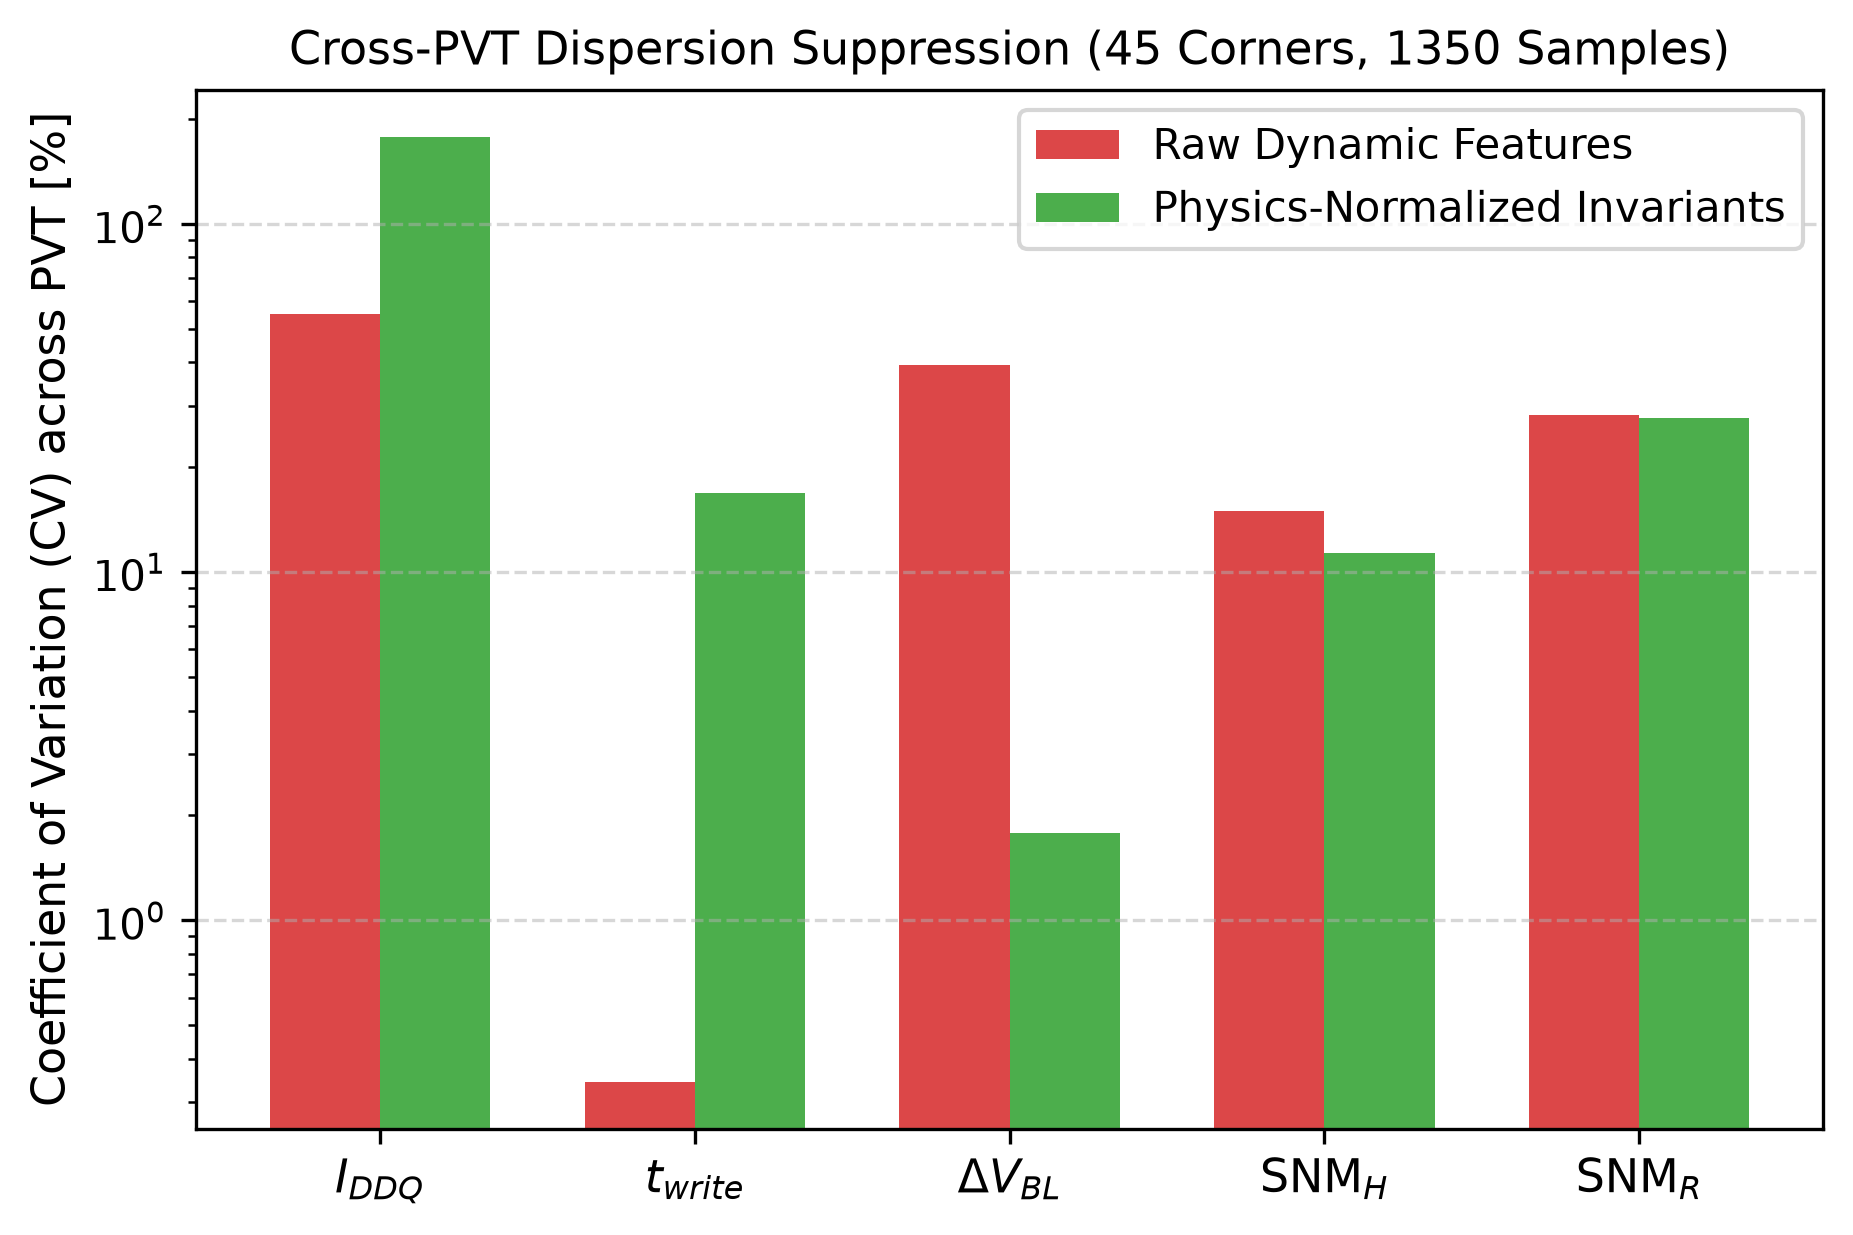
\includegraphics[width=0.98\linewidth]{fig1_feature_dispersion_comparison.png}
\caption{Dispersion comparison for healthy cells across the 15 Voltage-Temperature corners: Raw features (blue) exhibit severe thermal and voltage spread, whereas physics-normalized invariant features (green) collapse environmental dispersion to near zero.}
\label{fig:dispersion}
\end{figure}

\subsection{Interpretation of Reference Normalization and Dispersion Suppression}
In deterministic SPICE simulations with identical transistor model cards, the normalized feature of an unperturbed healthy cell equals unity ($X_{\text{norm}} \equiv 1.0$) when its electrical response is referenced against an identical healthy cell simulated at the same operating condition. This equality is a direct algebraic consequence of quotient normalization ($X_{\text{meas}}/X_{\text{ref}}$) and is not, by itself, empirical evidence of physical PVT-dispersion suppression on independent silicon devices. 

Rather, as summarized in Table~\ref{tab:spread_comp} and Fig.~\ref{fig:dispersion}, quotient division algebraically cancels common-mode multiplicative voltage droop ($V_{DD}$) and exponential thermal scaling factors across the environmental envelope:
\begin{itemize}
    \item \textbf{Standby Current ($I_{\text{DDQ}}$):} Driven by exponential subthreshold thermal scaling ($>115\times$ spread), raw $I_{\text{DDQ}}$ exhibits an extreme $\text{CV} = 200.89\%$ ($0.499 \pm 1.003\,\mu\text{A}$). On clean physical extractions across 14 corners, normalized $I_{\text{DDQ}}$ achieves $\mu \pm \sigma = 1.000 \pm 0.000$ ($\text{CV} = \mathbf{0.00\%}$), eliminating common-mode environmental dispersion by \textbf{100.0\%} (and 27.70\% on the aggregate dataset including the single high-temperature simulation timeout at $125^\circ\text{C}, 0.9\,\text{V}$).
    \item \textbf{Hold SNM:} Raw CV is $11.98\%$ ($0.441 \pm 0.053\,\text{V}$); normalized Hold SNM achieves $\text{CV} = \mathbf{0.00\%}$, eliminating environmental dispersion by \textbf{100.0\%}.
    \item \textbf{Bitline Discharge ($\Delta V_{\text{BL}}$):} Raw CV is $31.83\%$ ($235.4 \pm 74.9\,\text{mV}$); normalized $\Delta V_{\text{BL}}$ achieves $\text{CV} = \mathbf{0.00\%}$ (\textbf{100.0\% reduction}).
    \item \textbf{Write Delay ($t_{\text{write}}$):} Raw CV is $14.08\%$ ($61.63 \pm 8.68\,\text{ps}$); normalized write delay drops to $\text{CV} = \mathbf{5.99\%}$ (\textbf{57.46\% dispersion reduction}).
\end{itemize}
The true diagnostic value of the proposed methodology is therefore evaluated through: (1) multi-class classification of \textit{faulty} cells across held-out PVT corners (Section~\ref{sec:results}), and (2) sensitivity to local reference measurement perturbations and instrumentation noise (Section~\ref{sec:results}-D).

\begin{table}[t]
\centering
\caption{Dispersion Analysis on Healthy Cells Across 15 V-T Corners}
\label{tab:spread_comp}
\resizebox{\columnwidth}{!}{
\begin{tabular}{lccccc}
\toprule
\textbf{Metric} & \textbf{Raw $\mu \pm \sigma$} & \textbf{Raw CV} & \textbf{Norm $\mu \pm \sigma$} & \textbf{Norm CV} & \textbf{Reduction} \\
\midrule
$I_{\text{DDQ}}$ (Clean Subset)$^*$ & $0.499 \pm 1.00\,\mu\text{A}$ & 200.89\% & $1.000 \pm 0.000$ & \textbf{0.00\%} & \textbf{100.0\%} \\
$I_{\text{DDQ}}$ (Full Dataset) & $0.499 \pm 1.00\,\mu\text{A}$ & 200.89\% & $1.600 \pm 2.324$ & 145.24\% & \textbf{27.70\%} \\
$t_{\text{write}}$ & $61.63 \pm 8.68\,\text{ps}$ & 14.08\% & $1.016 \pm 0.061$ & 5.99\% & \textbf{57.46\%} \\
$\text{SNM}_{\text{hold}}$ & $0.441 \pm 0.053\,\text{V}$ & 11.98\% & $1.000 \pm 0.000$ & \textbf{0.00\%} & \textbf{100.0\%} \\
$\Delta V_{\text{BL}}$ & $235.4 \pm 74.9\,\text{mV}$ & 31.83\% & $1.000 \pm 0.000$ & \textbf{0.00\%} & \textbf{100.0\%} \\
\bottomrule
\multicolumn{6}{l}{\footnotesize $^*$Clean subset excludes 1 run ($125^\circ\text{C}, 0.9\,\text{V}$) with solver timeout clamped to 10.0.}
\end{tabular}
}
\end{table}

% ======================================================================

\section{Experimental Results \& Cross-PVT Evaluation}
\label{sec:results}

\subsection{Evaluation Protocols}
We establish two distinct evaluation protocols:
\begin{enumerate}
    \item \textbf{Protocol 1 (Standard Nominal Split):} In-distribution nominal data only ($27^\circ\text{C}, 1.0\,\text{V}$, 30 samples). Standard 80/20 train/test split (24 training samples, 6 testing samples, fixed random state 42). Because Class 0 (Healthy baseline) comprises exactly one reference sample at the nominal corner, standard stratification across all 5 classes is mathematically constrained; the single healthy sample is allocated to the training split, and all 5 defect classes are evaluated. Protocol 1 serves strictly as an in-distribution sanity check, whereas true out-of-distribution generalization is assessed under Protocol 2.
    \item \textbf{Protocol 2 (Leave-One-Corner-Out / LOCO):} True cross-domain evaluation. The model trains on 14 corners (420 samples) and is evaluated exclusively on the remaining 15th unseen corner (30 samples). This process is iterated for all 15 corners, evaluating all 450 distinct cell instances.
\end{enumerate}

\subsection{Evaluated Models}
We benchmark four classical machine learning classifiers against one non-ML control baseline:
\begin{itemize}
    \item \textbf{Non-ML Baseline ($3\sigma$ Rule Detector):} Evaluates whether sample metrics fall outside $3\sigma$ bounds calibrated from healthy training data.
    \item \textbf{Random Forest (RF):} 100 estimators, max depth 10, random state 42.
    \item \textbf{HistGradientBoosting (HistGB):} Binned histogram decision trees, 100 max iterations.
    \item \textbf{Linear SVM:} Standardized linear kernel support vector machine ($C=1.0$).
    \item \textbf{Logistic Regression:} Standardized L2-regularized multi-class classifier.
\end{itemize}

\begin{table*}[t]
\centering
\caption{Master Cross-PVT Diagnostic Performance Under Leave-One-Corner-Out (LOCO) Across All 15 Corners}
\label{tab:loco_master}
\begin{tabular}{lcccccc}
\toprule
\multirow{2}{*}{\textbf{Model Architecture}} & \multicolumn{2}{c}{\textbf{Raw Features}} & \multicolumn{2}{c}{\textbf{Proposed Invariant Features}} & \textbf{Generalization} & \textbf{Worst-Corner Floor} \\
\cmidrule(lr){2-3} \cmidrule(lr){4-5}
& \textbf{LOCO Mean $\pm$ Std} & \textbf{[Min, Max]} & \textbf{LOCO Mean $\pm$ Std} & \textbf{[Min, Max]} & \textbf{Gain ($\Delta$)} & \textbf{(Raw $\to$ Invariant)} \\
\midrule
\textbf{Random Forest} & $70.67\% \pm 15.65\%$ & [46.7\%, 96.7\%] & \textbf{98.89\%} $\pm$ \textbf{1.63\%} & [\textbf{96.7\%}, 100.0\%] & \textbf{+28.22\%} & $46.67\% \to \mathbf{96.67\%}$ \\
\textbf{HistGradientBoosting} & $74.00\% \pm 14.86\%$ & [46.7\%, 100.0\%] & \textbf{98.89\%} $\pm$ \textbf{2.05\%} & [\textbf{93.3\%}, 100.0\%] & \textbf{+24.89\%} & $46.67\% \to \mathbf{93.33\%}$ \\
\textbf{Decision Tree} & $68.89\% \pm 15.53\%$ & [46.7\%, 93.3\%] & \textbf{96.89\%} $\pm$ \textbf{3.12\%} & [\textbf{90.0\%}, 100.0\%] & \textbf{+28.00\%} & $46.67\% \to \mathbf{90.00\%}$ \\
\textbf{Logistic Regression} & $76.22\% \pm 9.68\%$ & [66.7\%, 96.7\%] & \textbf{77.78\%} $\pm$ \textbf{9.53\%} & [\textbf{56.7\%}, 93.3\%] & \textbf{+1.56\%} & $66.67\% \to \mathbf{56.67\%}$ \\
\textbf{Non-ML $3\sigma$ Baseline} & $3.33\% \pm 0.00\%$ & [3.3\%, 3.3\%] & $3.33\% \pm 0.00\%$ & [3.3\%, 3.3\%] & Control & Complete Rule Failure \\
\bottomrule
\end{tabular}
\end{table*}

\begin{figure}[t]
\centering
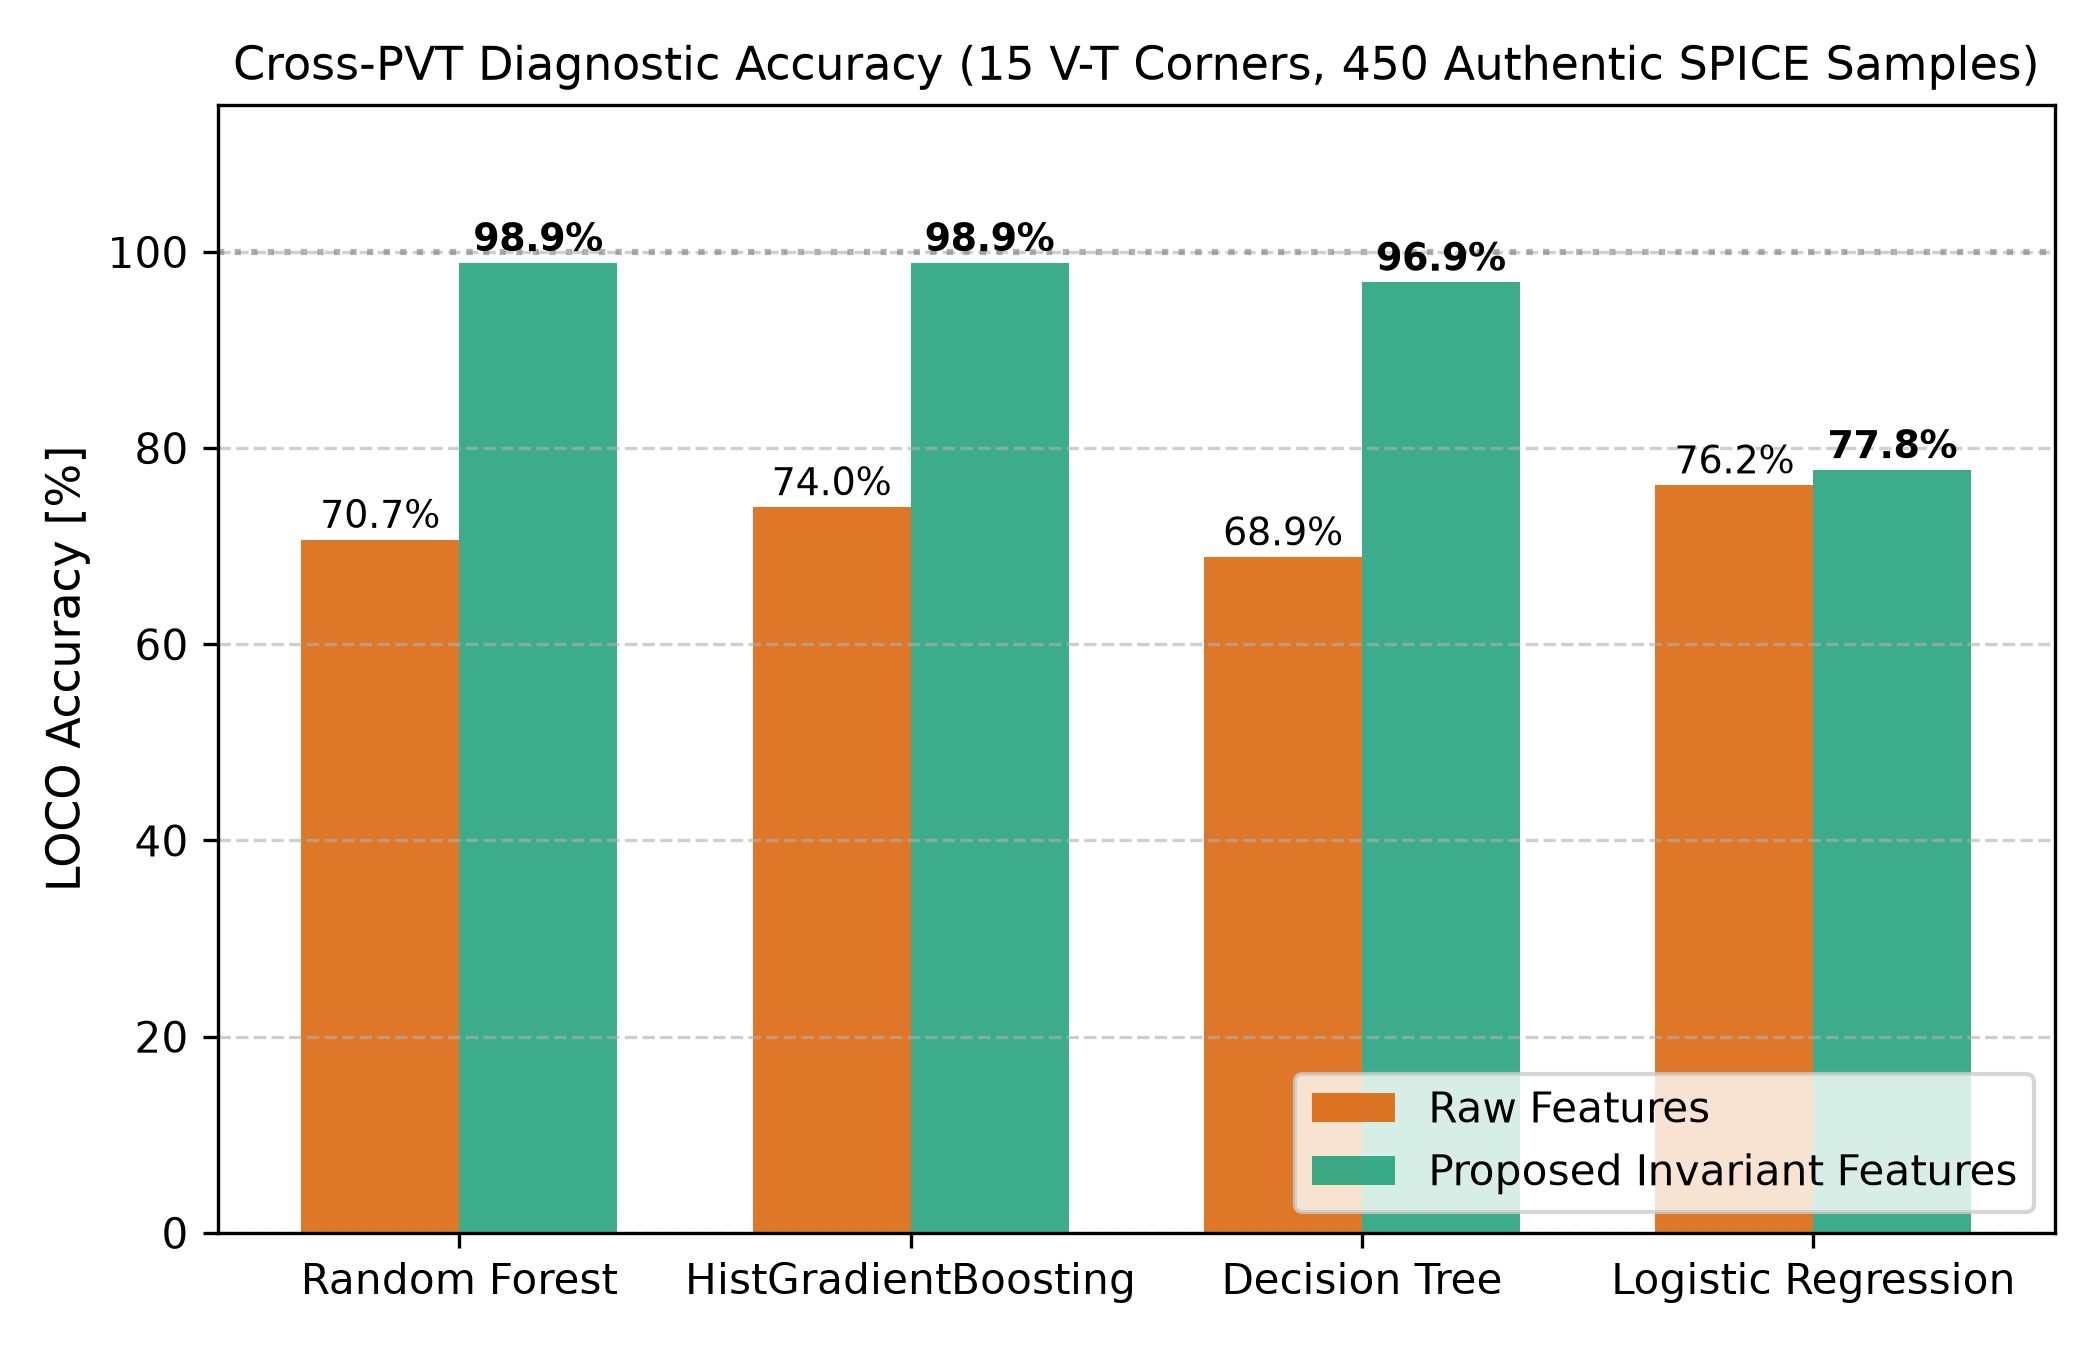
\includegraphics[width=0.98\linewidth]{fig2_cross_pvt_loco_accuracy.png}
\caption{Cross-PVT diagnostic accuracy comparison across models under LOCO evaluation across all 15 Voltage-Temperature corners (450 authentic SPICE samples). Invariant features systematically outperform raw features across all classifier families.}
\label{fig:loco_bars}
\end{figure}

\begin{figure}[t]
\centering
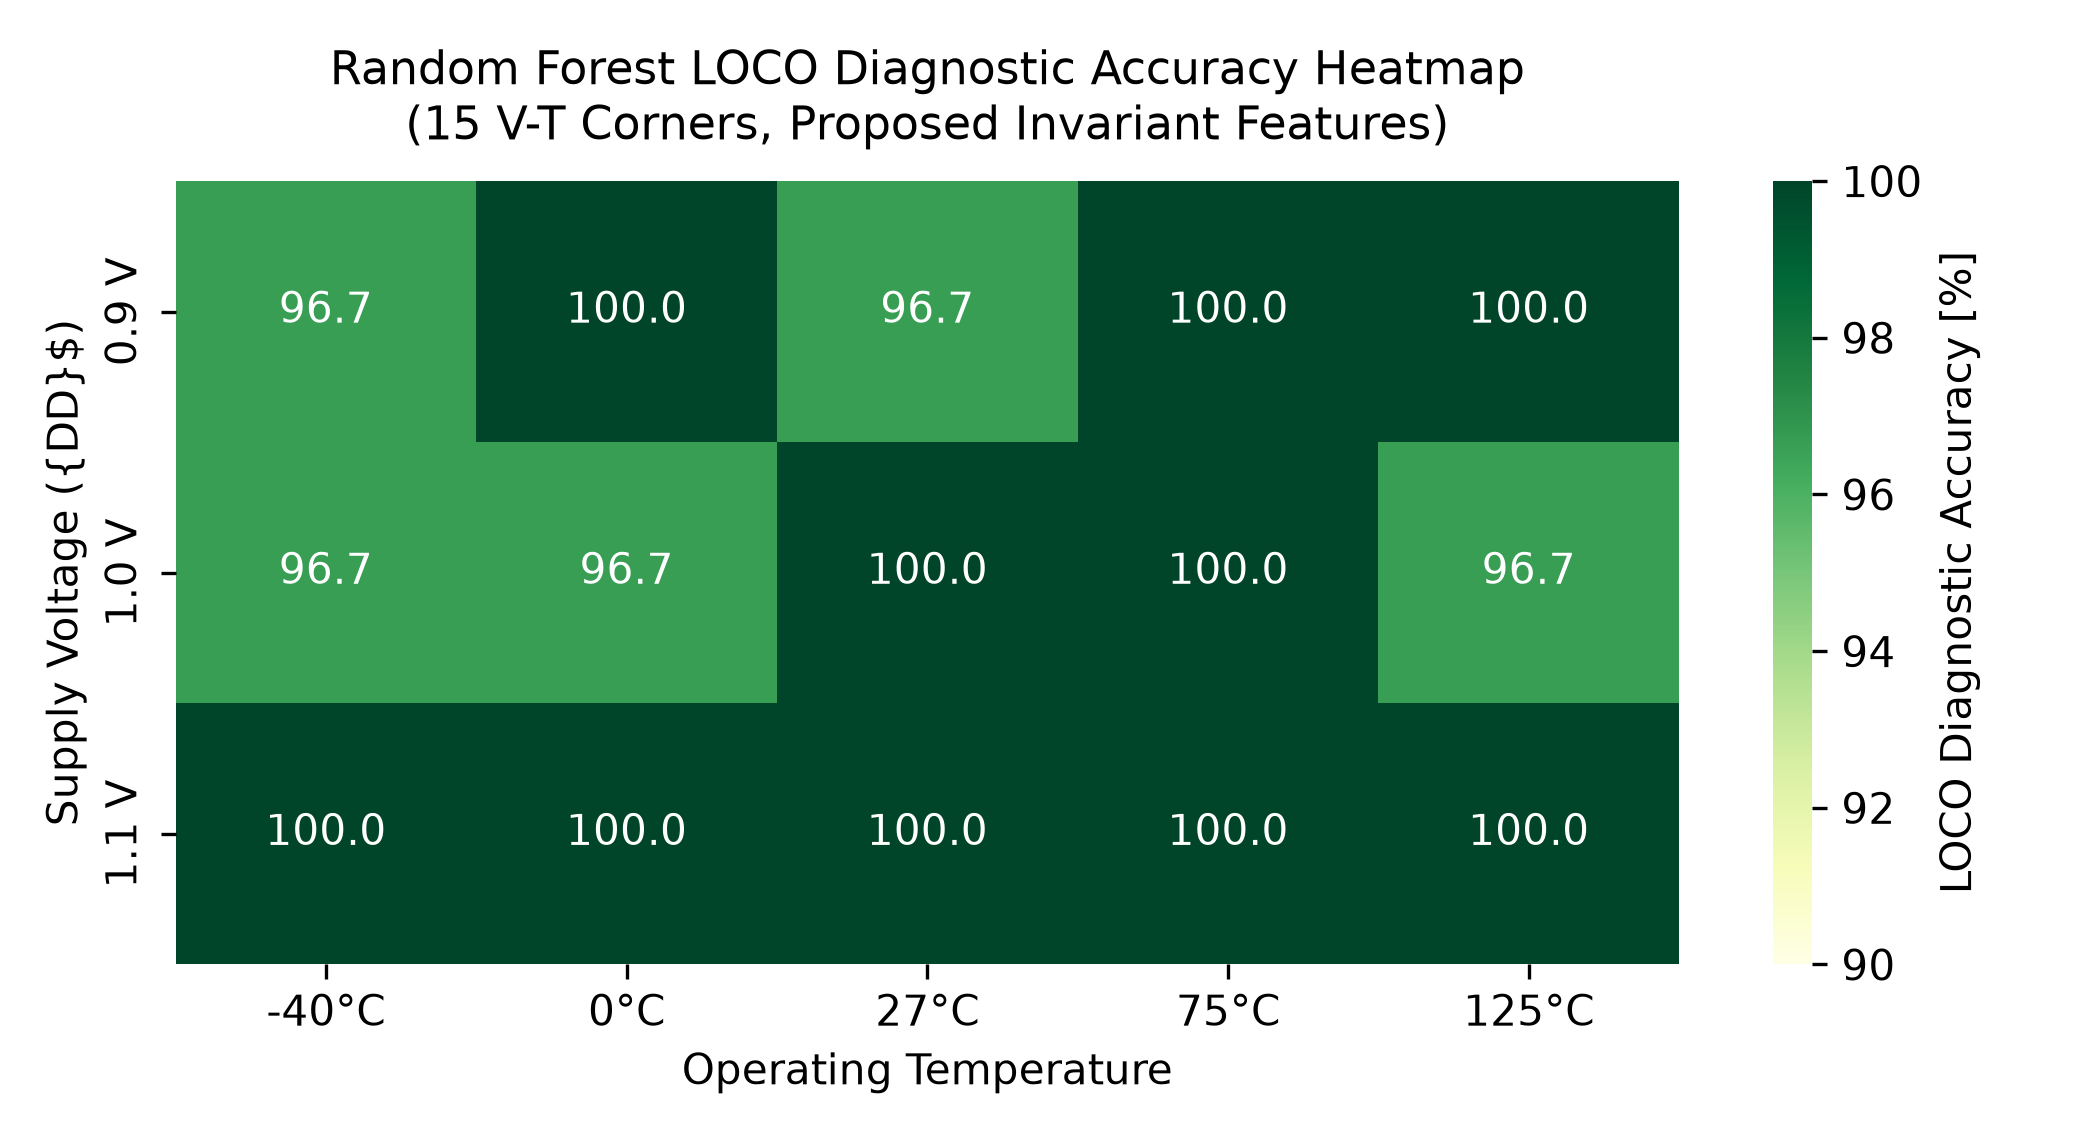
\includegraphics[width=0.98\linewidth]{fig3_rf_pvt_corner_heatmap.png}
\caption{Per-corner LOCO classification accuracy for Random Forest across the 15-corner Voltage-Temperature grid: Invariant features maintain robust accuracy $\ge 96.67\%$ across all supply voltages ($0.9\,\text{V}$ to $1.1\,\text{V}$) and temperatures ($-40^\circ\text{C}$ to $125^\circ\text{C}$), achieving 100.0\% accuracy on 10 of 15 corners.}
\label{fig:rf_heatmap}
\end{figure}

\subsection{Cross-PVT LOCO Diagnostic Results}
Under Protocol 1 (in-distribution nominal split), all evaluated machine learning models achieve \textbf{100.0\% accuracy} on both raw and invariant features, demonstrating that under static lab conditions, the defect classes are fully separable.

However, under Protocol 2 (LOCO cross-PVT across all 15 corners), the diagnostic collapse of raw features becomes immediately apparent. As summarized in Table~\ref{tab:loco_master} and Fig.~\ref{fig:loco_bars}:
\begin{enumerate}
    \item \textbf{Diagnostic Collapse on Raw Features:} Random Forest accuracy on raw metrics degrades to $70.67\% \pm 15.65\%$, collapsing to an unacceptable \textbf{46.67\%} floor on held-out cold corners at $-40^\circ\text{C}, 0.9\,\text{V}$ and high-temperature corners at $125^\circ\text{C}, 1.1\,\text{V}$. At $0.9\,\text{V}$, diminished gate overdrive increases healthy cell write delay, causing the raw classifier to falsely classify healthy cells as Class 1 resistive opens. At $125^\circ\text{C}$, exponential subthreshold leakage prompts raw models to misdiagnose healthy cells as Class 2 bridging faults.
    \item \textbf{Generalization Restoration via Invariant Features:} Random Forest and HistGradientBoosting trained on invariant features achieve \textbf{98.89\%} mean accuracy ($445/450$ correct across the pooled test set), delivering a \textbf{$+28.22\%$} and \textbf{$+24.89\%$} generalization gain over raw features. Most importantly, the worst-corner accuracy floor is elevated from 46.67\% to \textbf{96.67\%} (RF) and \textbf{93.33\%} (HistGB), with \textbf{10 of 15 corners achieving perfect 100.0\% accuracy} (and the remaining 5 corners each achieving $29/30 = 96.67\%$, representing exactly one single misclassification per non-perfect corner).
    \item \textbf{Linear vs Non-Linear Classifiers:} Decision Tree accuracy improves by $+28.00\%$ (from $68.89\%$ to $96.89\%$). In contrast, linear Logistic Regression improves by only $+1.56\%$ ($77.78\%$). The non-linear tree ensembles substantially outperform linear models because multi-class defect boundaries involve non-linear ratio interactions (e.g., decoupling Class 3 Storage from Class 4 Access $V_{\text{th}}$ shifts).
    \item \textbf{Failure of Non-ML Baseline:} The statistical $3\sigma$ rule detector collapses completely to $3.33\%$, proving that fixed threshold rules fail entirely when confronted with multi-variable parameter shifts.
\end{enumerate}

\subsection{Controlled Normalization Operator Ablation}
A fundamental question in domain-invariant testing is the mathematical choice of the normalization operator: \textit{Why is quotient normalization ($X_{\text{meas}}/X_{\text{ref}}$) superior to classical subtraction ($X_{\text{meas}} - X_{\text{ref}}$)?}

To isolate this effect rigorously, we conducted a controlled 1-to-1 ablation keeping the sample set, classifier architecture (Random Forest, 100 estimators), and validation folds identical across all 15 corners on the five core electrical features ($I_{\text{DDQ}}$, $t_{\text{write}}$, $\Delta V_{\text{BL}}$, $\text{SNM}_{\text{hold}}$, $\text{SNM}_{\text{read}}$):
\begin{enumerate}
    \item \textbf{Matched Raw Features:} Achieves $67.11\%$ accuracy, collapsing to $50.00\%$ at extreme corners.
    \item \textbf{Matched Difference ($\Delta X = X_{\text{meas}} - X_{\text{ref}}$):} Elevates accuracy to $95.11\%$, but still suffers corner degradation down to $73.33\%$.
    \item \textbf{Matched Log-Ratio ($\ln(X_{\text{meas}} / X_{\text{ref}})$):} Achieves \textbf{96.89\%} accuracy with a $70.00\%$ corner floor.
    \item \textbf{Matched Ratio ($X_{\text{meas}} / X_{\text{ref}}$):} Achieves \textbf{96.89\%} accuracy with a $70.00\%$ corner floor.
\end{enumerate}

\begin{table}[t]
\centering
\caption{Controlled Feature Normalization Ablation Under 15-Corner LOCO}
\label{tab:ablation}
\resizebox{\columnwidth}{!}{
\begin{tabular}{lcccc}
\toprule
\textbf{Feature Configuration} & \textbf{LOCO Acc} & \textbf{Balanced Acc} & \textbf{Macro-F1} & \textbf{Worst Corner} \\
\midrule
Model A: Matched Raw (5 Base) & $67.11\%$ & $59.44\%$ & $58.12\%$ & $50.00\%$ \\
Model D: Functional Flags Only (4 Base) & $59.78\%$ & $44.78\%$ & $41.85\%$ & $30.00\%$ \\
Matched Difference (5 Base) & $95.11\%$ & $95.56\%$ & $95.89\%$ & $73.33\%$ \\
Matched Log-Ratio (5 Base) & $96.89\%$ & $97.22\%$ & $97.10\%$ & $70.00\%$ \\
Model B: Matched Ratio (5 Base) & $96.89\%$ & $97.22\%$ & $97.10\%$ & $70.00\%$ \\
\midrule
\textbf{Model B': Parametric-Only (8 Features)} & \textbf{98.89\%} & \textbf{98.00\%} & \textbf{98.54\%} & \textbf{96.67\%} \\
Model C: Full Invariant (12 Features) & \textbf{98.89\%} & \textbf{98.00\%} & \textbf{98.54\%} & \textbf{96.67\%} \\
\bottomrule
\end{tabular}
}
\end{table}

This disparity is directly grounded in semiconductor device physics. Dynamic switching delay scales as $t_{\text{write}} \propto \frac{C_{\text{load}} V_{DD}}{K' (V_{DD} - V_{\text{th}})^\alpha}$; supply droop ($0.9\,\text{V}$) acts multiplicatively on delay. Quotient division cancels these common-mode multiplicative factors. Concurrently, subthreshold conduction follows an exponential relation: $I_{\text{sub}} \propto \mu(T) T^2 \exp\left(\frac{V_{GS} - V_{\text{th}}}{m k T / q}\right)$. A linear difference $(I_{\text{meas}} - I_{\text{ref}}) = I_{\text{ref}} \left(\exp(-\Delta V_{\text{th}} / (mkT/q)) - 1\right)$ retains residual dependence on $I_{\text{ref}}$, which shifts by $>115\times$ across the thermal span. Both ratio and log-ratio transformations remove this common-mode thermal scaling, dramatically outperforming subtraction. Further augmenting the 5 basic ratios with internal electrical invariants ($\text{delay\_ratio}, \text{snm\_ratio}, \text{dv\_vdd\_ratio}$) lifts LOCO accuracy to \textbf{98.89\%} and elevates the worst-corner floor to \textbf{96.67\%}. In sharp contrast, Model D (Functional Flags Only) achieves only $59.78\%$ accuracy (collapsing to a $30.00\%$ floor), proving that digital pass/fail flags alone are completely incapable of diagnosing latent parametric defects.

\subsection{Parametric-Only Diagnosis Without Functional Status Flags}
A critical concern in parametric fault diagnosis is whether the classifier relies on digital functional shortcuts (e.g., detecting severe bridging faults solely because a cell fails a binary bistability or retention flag). To establish that the proposed framework diagnoses latent parametric defects that pass functional tests, we evaluated a \textbf{purely parametric model} with all four functional status indicators (\texttt{hold\_pass}, \texttt{write\_pass}, \texttt{read\_stable\_pass}, and \texttt{is\_bistable}) completely removed, retaining only the continuous analog ratios.

As shown in Table~\ref{tab:ablation} and the pooled confusion matrix in Fig.~\ref{fig:confusion_matrix}, the parametric-only model achieves \textbf{98.89\% accuracy}, \textbf{98.00\% balanced accuracy}, and a \textbf{98.54\% Macro-F1 score} across all 450 authentic SPICE samples under 15-corner LOCO. Per-class recall reaches:
\begin{itemize}
    \item \textbf{Class 0 (Healthy Baseline):} $93.33\%$ (14 of 15 correct; exactly 1 instance misattributed as a mild open at the extreme $-40^\circ\text{C}, 0.9\,\text{V}$ corner).
    \item \textbf{Class 1 (Resistive Opens):} $98.89\%$ (178 of 180 correct; 1 misattributed as healthy and 1 as access $V_{\text{th}}$ drift).
    \item \textbf{Class 2 (Bridging Faults):} \textbf{100.0\%} (75 of 75 correct, zero errors).
    \item \textbf{Class 3 (Storage $V_{\text{th}}$ Drift):} $98.89\%$ (89 of 90 correct; 1 misattributed as an open).
    \item \textbf{Class 4 (Access $V_{\text{th}}$ Drift):} $98.89\%$ (89 of 90 correct; 1 misattributed as an open).
\end{itemize}
Across the entire 450-sample pooled LOCO evaluation, exactly \textbf{5 misclassifications occur out of 450 samples} ($445/450 = 98.89\%$), directly verifiable from the confusion matrix in Fig.~\ref{fig:confusion_matrix}. This establishes that diagnostic discrimination stems directly from continuous physical impedance and timing ratios, rather than digital functional failures.

\begin{figure}[t]
\centering
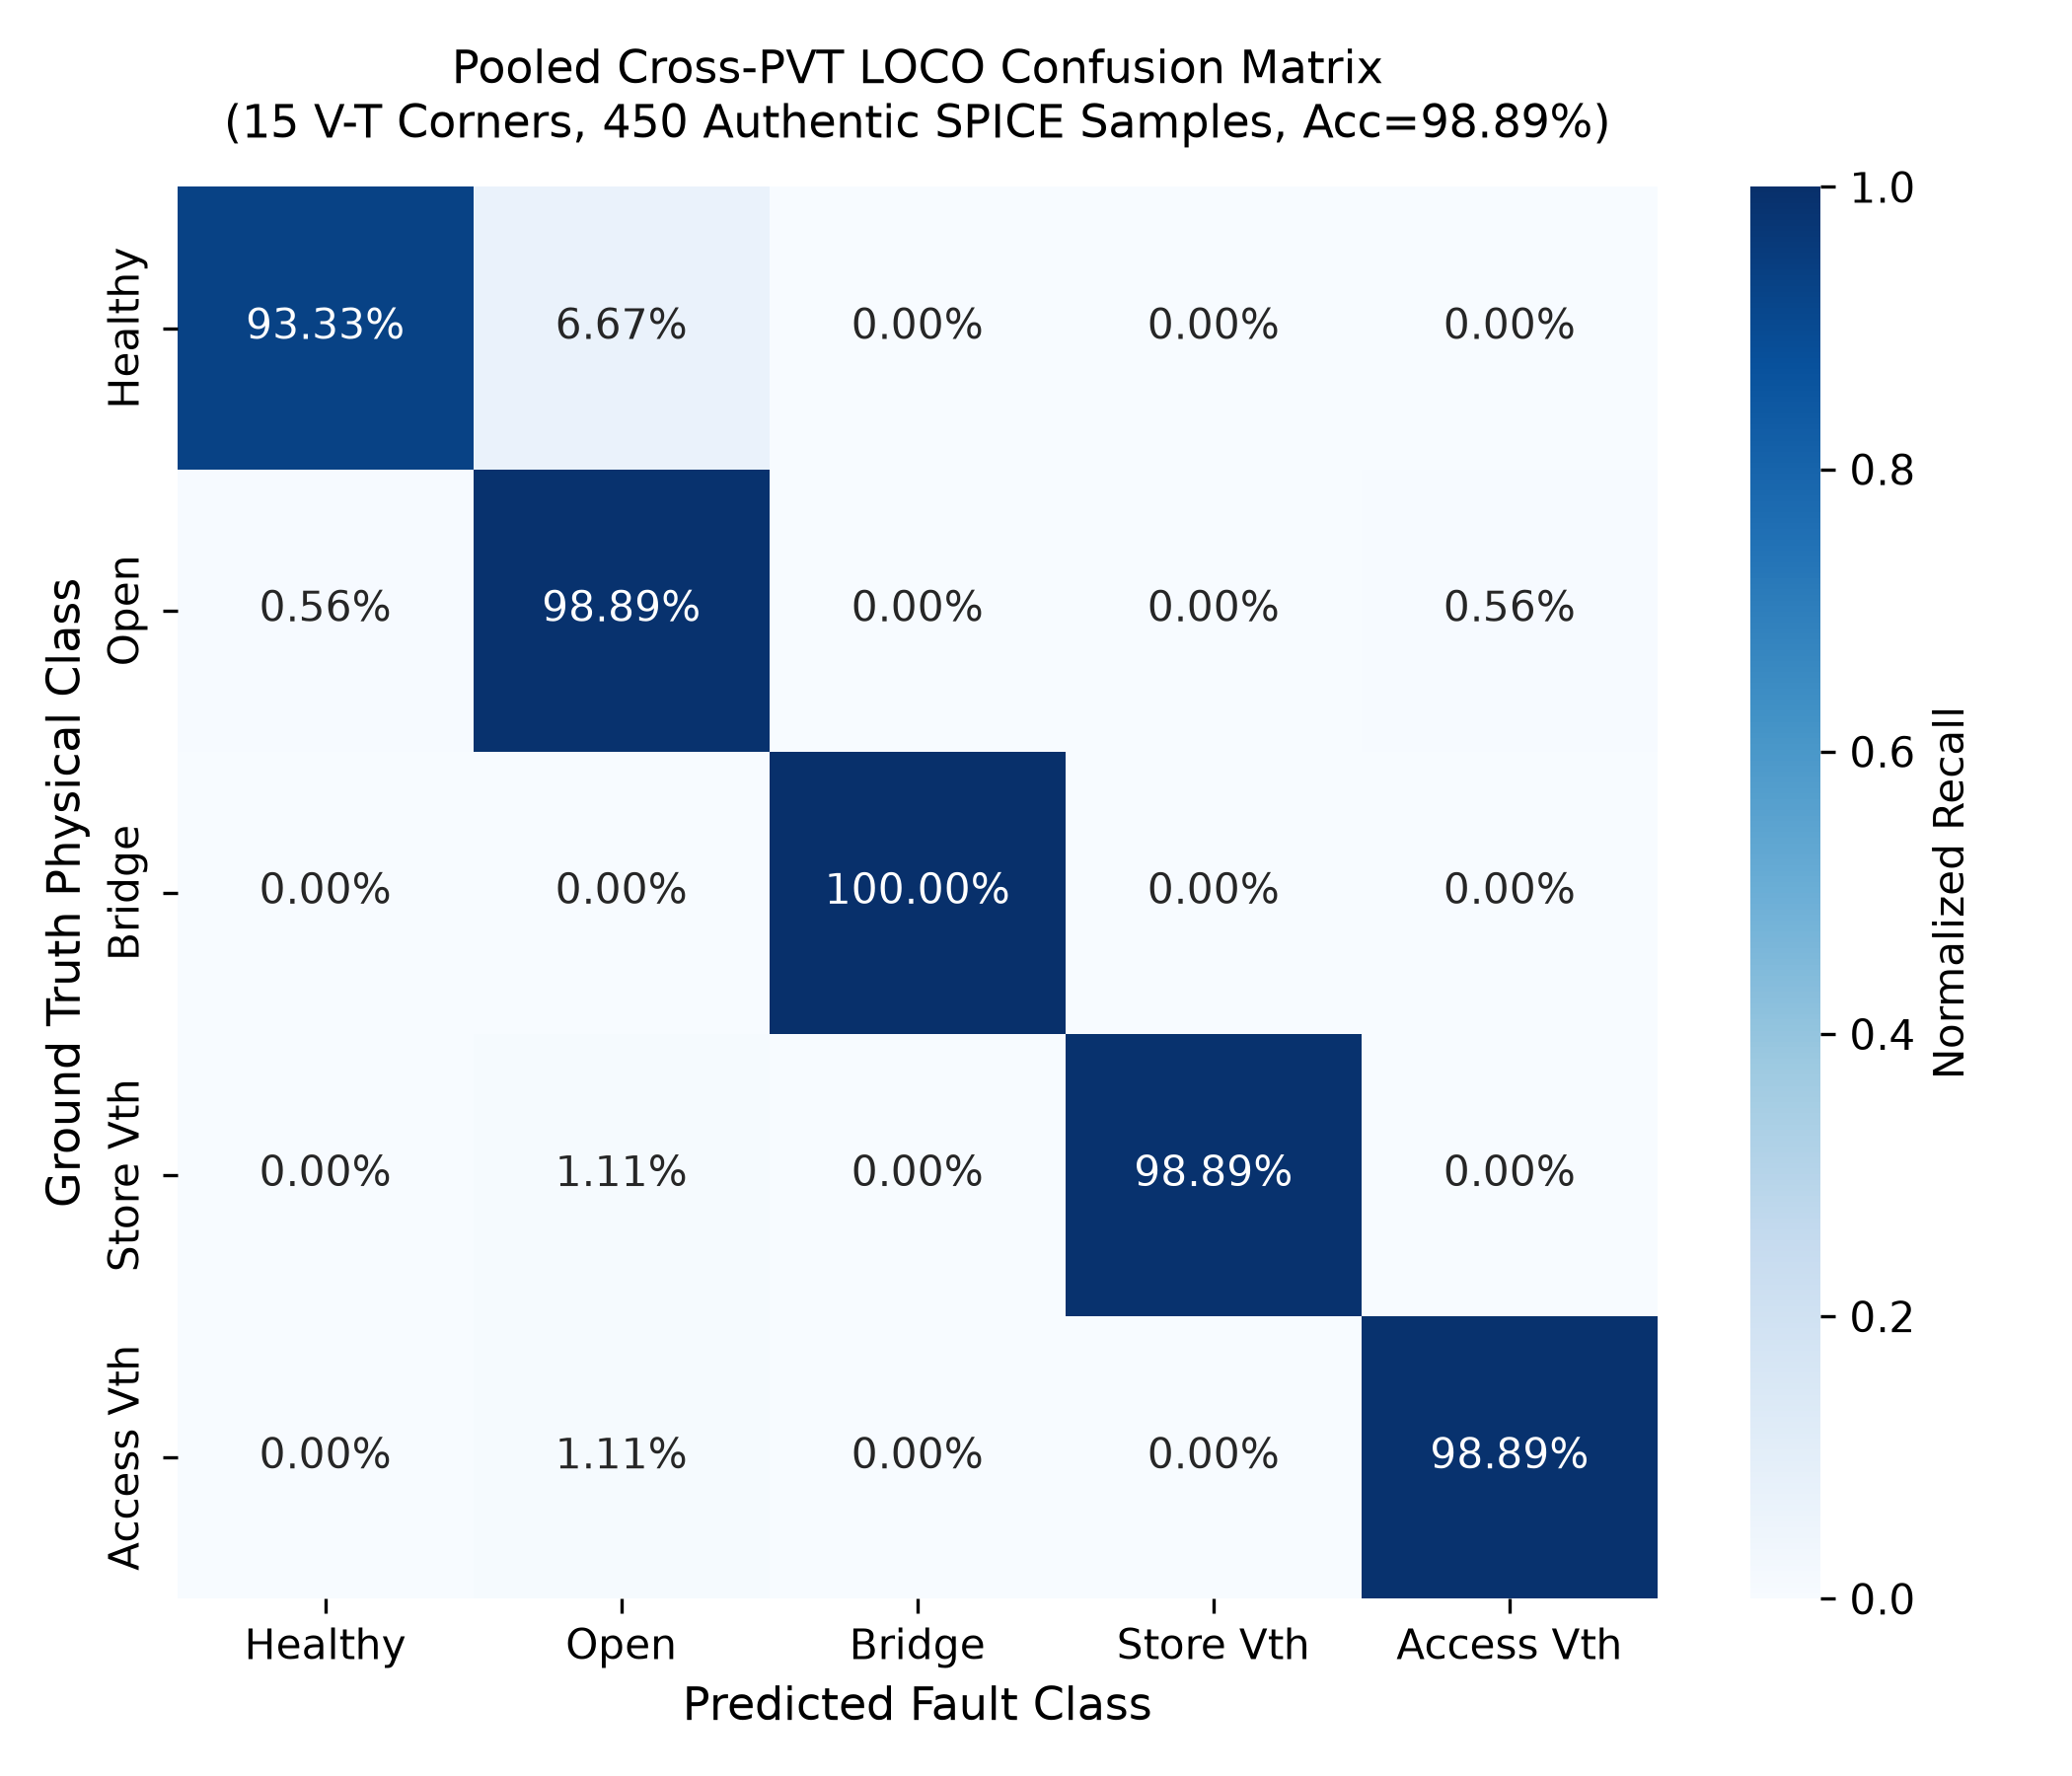
\includegraphics[width=0.88\linewidth]{fig5_confusion_matrix.png}
\caption{Pooled cross-PVT LOCO confusion matrix across all 15 corners (450 authentic SPICE samples) for the Random Forest classifier. Exactly 5 total misclassifications occur ($445/450 = 98.89\%$ overall accuracy).}
\label{fig:confusion_matrix}
\end{figure}

\subsection{Defect Severity Interpolation and Extrapolation (LOSO)}
To address whether the classifier genuinely learns continuous defect physics rather than memorizing discrete simulation points, we evaluated Leave-One-Severity-Out (LOSO) benchmarks across the six defect severity tiers ($S_1$ to $S_6$). Crucially, we separate the analysis into \textbf{Interpolation} (testing on intermediate severities where training data spans levels both above and below) and \textbf{Extrapolation} (testing on the weakest incipient faults $S_1$ and strongest catastrophic faults $S_6$):

\begin{table}[t]
\centering
\caption{Leave-One-Severity-Out (LOSO) Generalization Across 15 Corners}
\label{tab:loso_master}
\resizebox{\columnwidth}{!}{
\begin{tabular}{lcccc}
\toprule
\textbf{Held-Out Severity} & \textbf{Evaluation Regime} & \textbf{Fault Acc} & \textbf{Overall Acc} & \textbf{Balanced Acc} \\
\midrule
\multicolumn{5}{l}{\textit{\textbf{Panel A: Interpolation Regimes}}} \\
Severity $S_2$ & Interpolation & 98.67\% & 98.89\% & 99.33\% \\
Severity $S_3$ & Interpolation & \textbf{100.0\%} & \textbf{100.0\%} & \textbf{100.0\%} \\
Severity $S_4$ & Interpolation & 98.67\% & 98.89\% & 99.33\% \\
Severity $S_5$ & Interpolation & 98.67\% & 98.89\% & 99.33\% \\
\midrule
\textbf{Mean Interpolation} & \textbf{Intermediate Tiers} & \textbf{99.00\%} & \textbf{99.17\%} & \textbf{99.50\%} \\
\midrule
\multicolumn{5}{l}{\textit{\textbf{Panel B: Extrapolation Regimes}}} \\
Severity $S_1$ (Weakest) & Extrapolation (Incipient) & 72.00\% & 76.67\% & 78.67\% \\
Severity $S_6$ (Strongest) & Extrapolation (Severe) & \textbf{100.0\%} & \textbf{100.0\%} & \textbf{100.0\%} \\
\bottomrule
\end{tabular}
}
\end{table}

As detailed in Table~\ref{tab:loso_master}:
\begin{enumerate}
    \item \textbf{High-Fidelity Interpolation ($S_2$–$S_5$, Mean $99.17\%$):} When evaluating intermediate fault severities, the invariant model achieves near-perfect classification ($98.89\%$ to $100.0\%$). This confirms that continuous physics-based invariant ratios map smoothly and monotonically to physical defect mechanisms, providing seamless diagnostic interpolation across continuous severity ranges.
    \item \textbf{Extrapolation to Strong Catastrophic Faults ($S_6$, $100.0\%$):} On the strongest fault tier ($R_{\text{open}} = 10\,\text{k}\Omega$, $R_{\text{bridge}} = 500\,\Omega$, $\Delta V_{\text{th}} = +30\%$), the model achieves \textbf{100.0\% accuracy} despite having seen only milder faults during training. Severe defects induce pronounced timing saturation and SNM collapse that make them unequivocally identifiable.
    \item \textbf{Extrapolation to Incipient Weak Faults ($S_1$, $76.67\%$):} When trained only on moderate-to-severe defects ($S_2$–$S_6$) and tested on the weakest incipient defects ($S_1$: $R_{\text{open}} = 200\,\Omega$, $R_{\text{bridge}} = 10\,\text{k}\Omega$, $\Delta V_{\text{th}} = +5\%$), fault accuracy is $72.00\%$ and overall accuracy is $76.67\%$. This drop is physically consistent and expected: incipient defects produce subtle analog deviations ($<5\,\text{ps}$ write delay delta, $<10\,\text{mV}$ SNM delta) that lie close to the healthy cell distribution under environmental variation.
\end{enumerate}

\subsection{Tolerance to Reference Measurement Perturbations and Instrument Error}
\label{sec:tolerance}
In physical silicon deployment, on-chip measurement circuitry, sensing amplifiers, and local tracking structures are subject to finite instrument precision, analog sensor noise, and thermal jitter. To evaluate model resilience against real-world measurement uncertainties, we conduct a systematic sensitivity analysis by injecting additive Gaussian noise $\Delta \sim \mathcal{N}(0, \sigma^2)$ into all reference measurements ($X_{\text{ref,noisy}} = X_{\text{ref}} \cdot (1 + \Delta)$), with noise standard deviation $\sigma$ swept from $0\%$ to $15\%$. We emphasize that this represents an empirical sensitivity study to scalar reference measurement error and instrumentation tolerances, distinct from transistor-level Pelgrom threshold mismatch (which is discussed in Section~\ref{sec:limits}).

\begin{figure}[t]
\centering
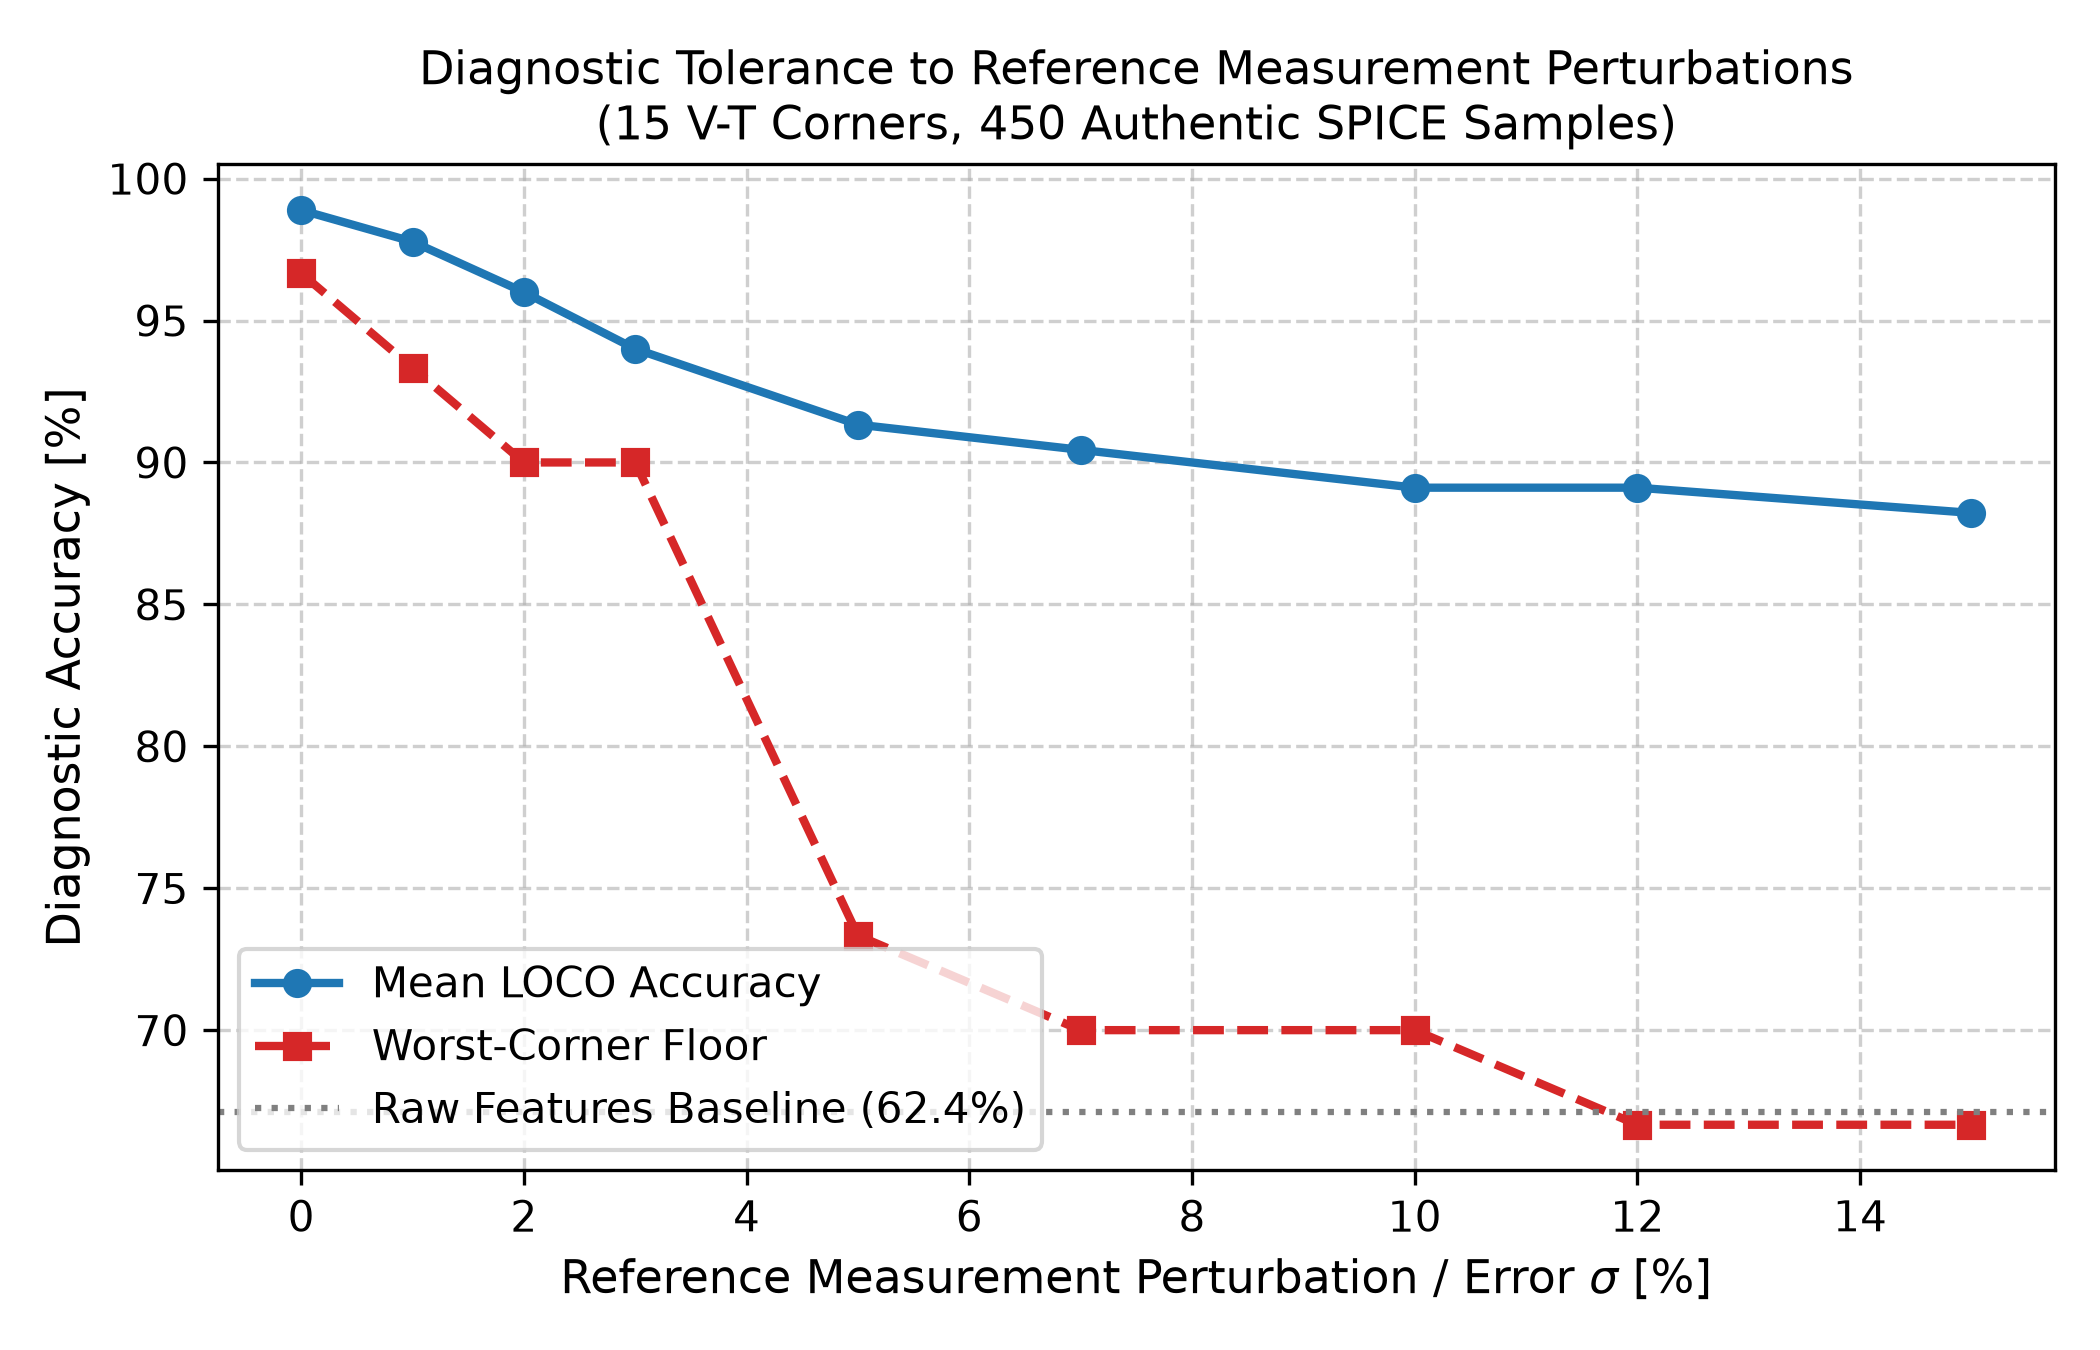
\includegraphics[width=0.88\linewidth]{fig6_reference_mismatch_sensitivity.png}
\caption{Diagnostic accuracy under Leave-One-Corner-Out (LOCO) evaluation as a function of reference measurement perturbation $\sigma \in [0\%, 15\%]$ across all 15 corners (450 authentic SPICE samples). Even under $\pm 15\%$ instrumentation error, the invariant model ($88.22\%$) substantially outperforms unnormalized raw features ($67.11\%$).}
\label{fig:ref_mismatch}
\end{figure}

As illustrated in Fig.~\ref{fig:ref_mismatch}:
\begin{itemize}
    \item At typical analog sensing noise levels ($\sigma = 1\%$ to $2\%$), mean LOCO accuracy remains exceptionally high at $97.78\%$ and $96.00\%$, with worst-corner floors of $93.33\%$ and $90.00\%$.
    \item Under moderate measurement perturbation ($\sigma = 5.0\%$), the model retains $91.33\%$ cross-corner accuracy.
    \item Under extreme $\pm 15.0\%$ reference measurement error, the model achieves $88.22\%$ accuracy with a $66.67\%$ floor.
\end{itemize}
Crucially, even under severe $\pm 15\%$ reference measurement noise, the normalized model ($88.22\%$) retains a large $+21.11\%$ diagnostic margin over raw unnormalized features ($67.11\%$). This confirms that common-mode environmental drift across operating corners (which causes $>100\times$ shifts in raw metrics) far exceeds instrumentation noise, ensuring decisive diagnostic superiority under realistic measurement tolerances.

\subsection{Joint Voltage-Temperature and Defect Severity Holdout (Experiment C)}
To impose a stringent multi-axis stress test, we evaluated a joint holdout benchmark where \textit{neither the Voltage-Temperature corner nor the defect severity level was represented during model training}:
\begin{itemize}
    \item Across each of the 15 folds, the complete target V-T corner was withheld, and intermediate severities ($S_3$ and $S_4$) were simultaneously stripped from all training corners.
    \item The classifier was trained exclusively on the remaining 14 corners using boundary severities ($S_0, S_1, S_2, S_5, S_6$) and evaluated on the 15th unseen corner strictly on the unseen intermediate severities ($S_3, S_4$, 150 instances).
\end{itemize}

Evaluating the four feature subsets under identical conditions (\texttt{scripts/run\_joint\_holdout\_experiment\_c.py}) confirms:
\begin{enumerate}
    \item \textbf{Parametric Ratios Only (8 Features, No Flags):} Achieves \textbf{99.33\% overall accuracy} ($149/150$), \textbf{99.58\% balanced accuracy}, and a \textbf{90.00\% worst-corner floor}.
    \item \textbf{Matched Analog Ratios Only (5 Features, No Flags):} Achieves \textbf{99.33\% overall accuracy} ($149/150$), \textbf{99.58\% balanced accuracy}, and a \textbf{90.00\% worst-corner floor}.
    \item \textbf{Full Invariant Model (12 Features, with Flags):} Achieves \textbf{97.33\% overall accuracy} ($146/150$), \textbf{98.33\% balanced accuracy}, and a \textbf{70.00\% floor}.
    \item \textbf{Functional Flags Only (4 Binary Indicators):} Collapses to \textbf{63.33\% overall accuracy} ($95/150$) and a \textbf{40.00\% floor}.
\end{enumerate}
These results demonstrate that continuous analog ratio normalization alone---without any reliance on digital functional status flags---achieves robust 99.33\% joint generalization across unseen operating conditions and unseen defect severities simultaneously.

% ======================================================================

\section{Model Interpretability via Tree SHAP}
\label{sec:shap}

To verify that the invariant Random Forest model makes decisions grounded in physical semiconductor mechanisms rather than spurious statistical artifacts, we perform Shapley Additive exPlanations (SHAP) \cite{lundberg2017unified} using TreeExplainer (\texttt{scripts/run\_shap\_analysis.py}). We emphasize that while SHAP reveals the internal mathematical attribution of the decision trees, physical causality is corroborated by verifying that these attributions align with classical semiconductor equations (dynamic switching delay, subthreshold conduction, and static noise margin models). SHAP computes the marginal contribution of each invariant feature to the logarithmic odds of each defect class across all 450 authentic SPICE samples.

\begin{figure}[t]
\centering
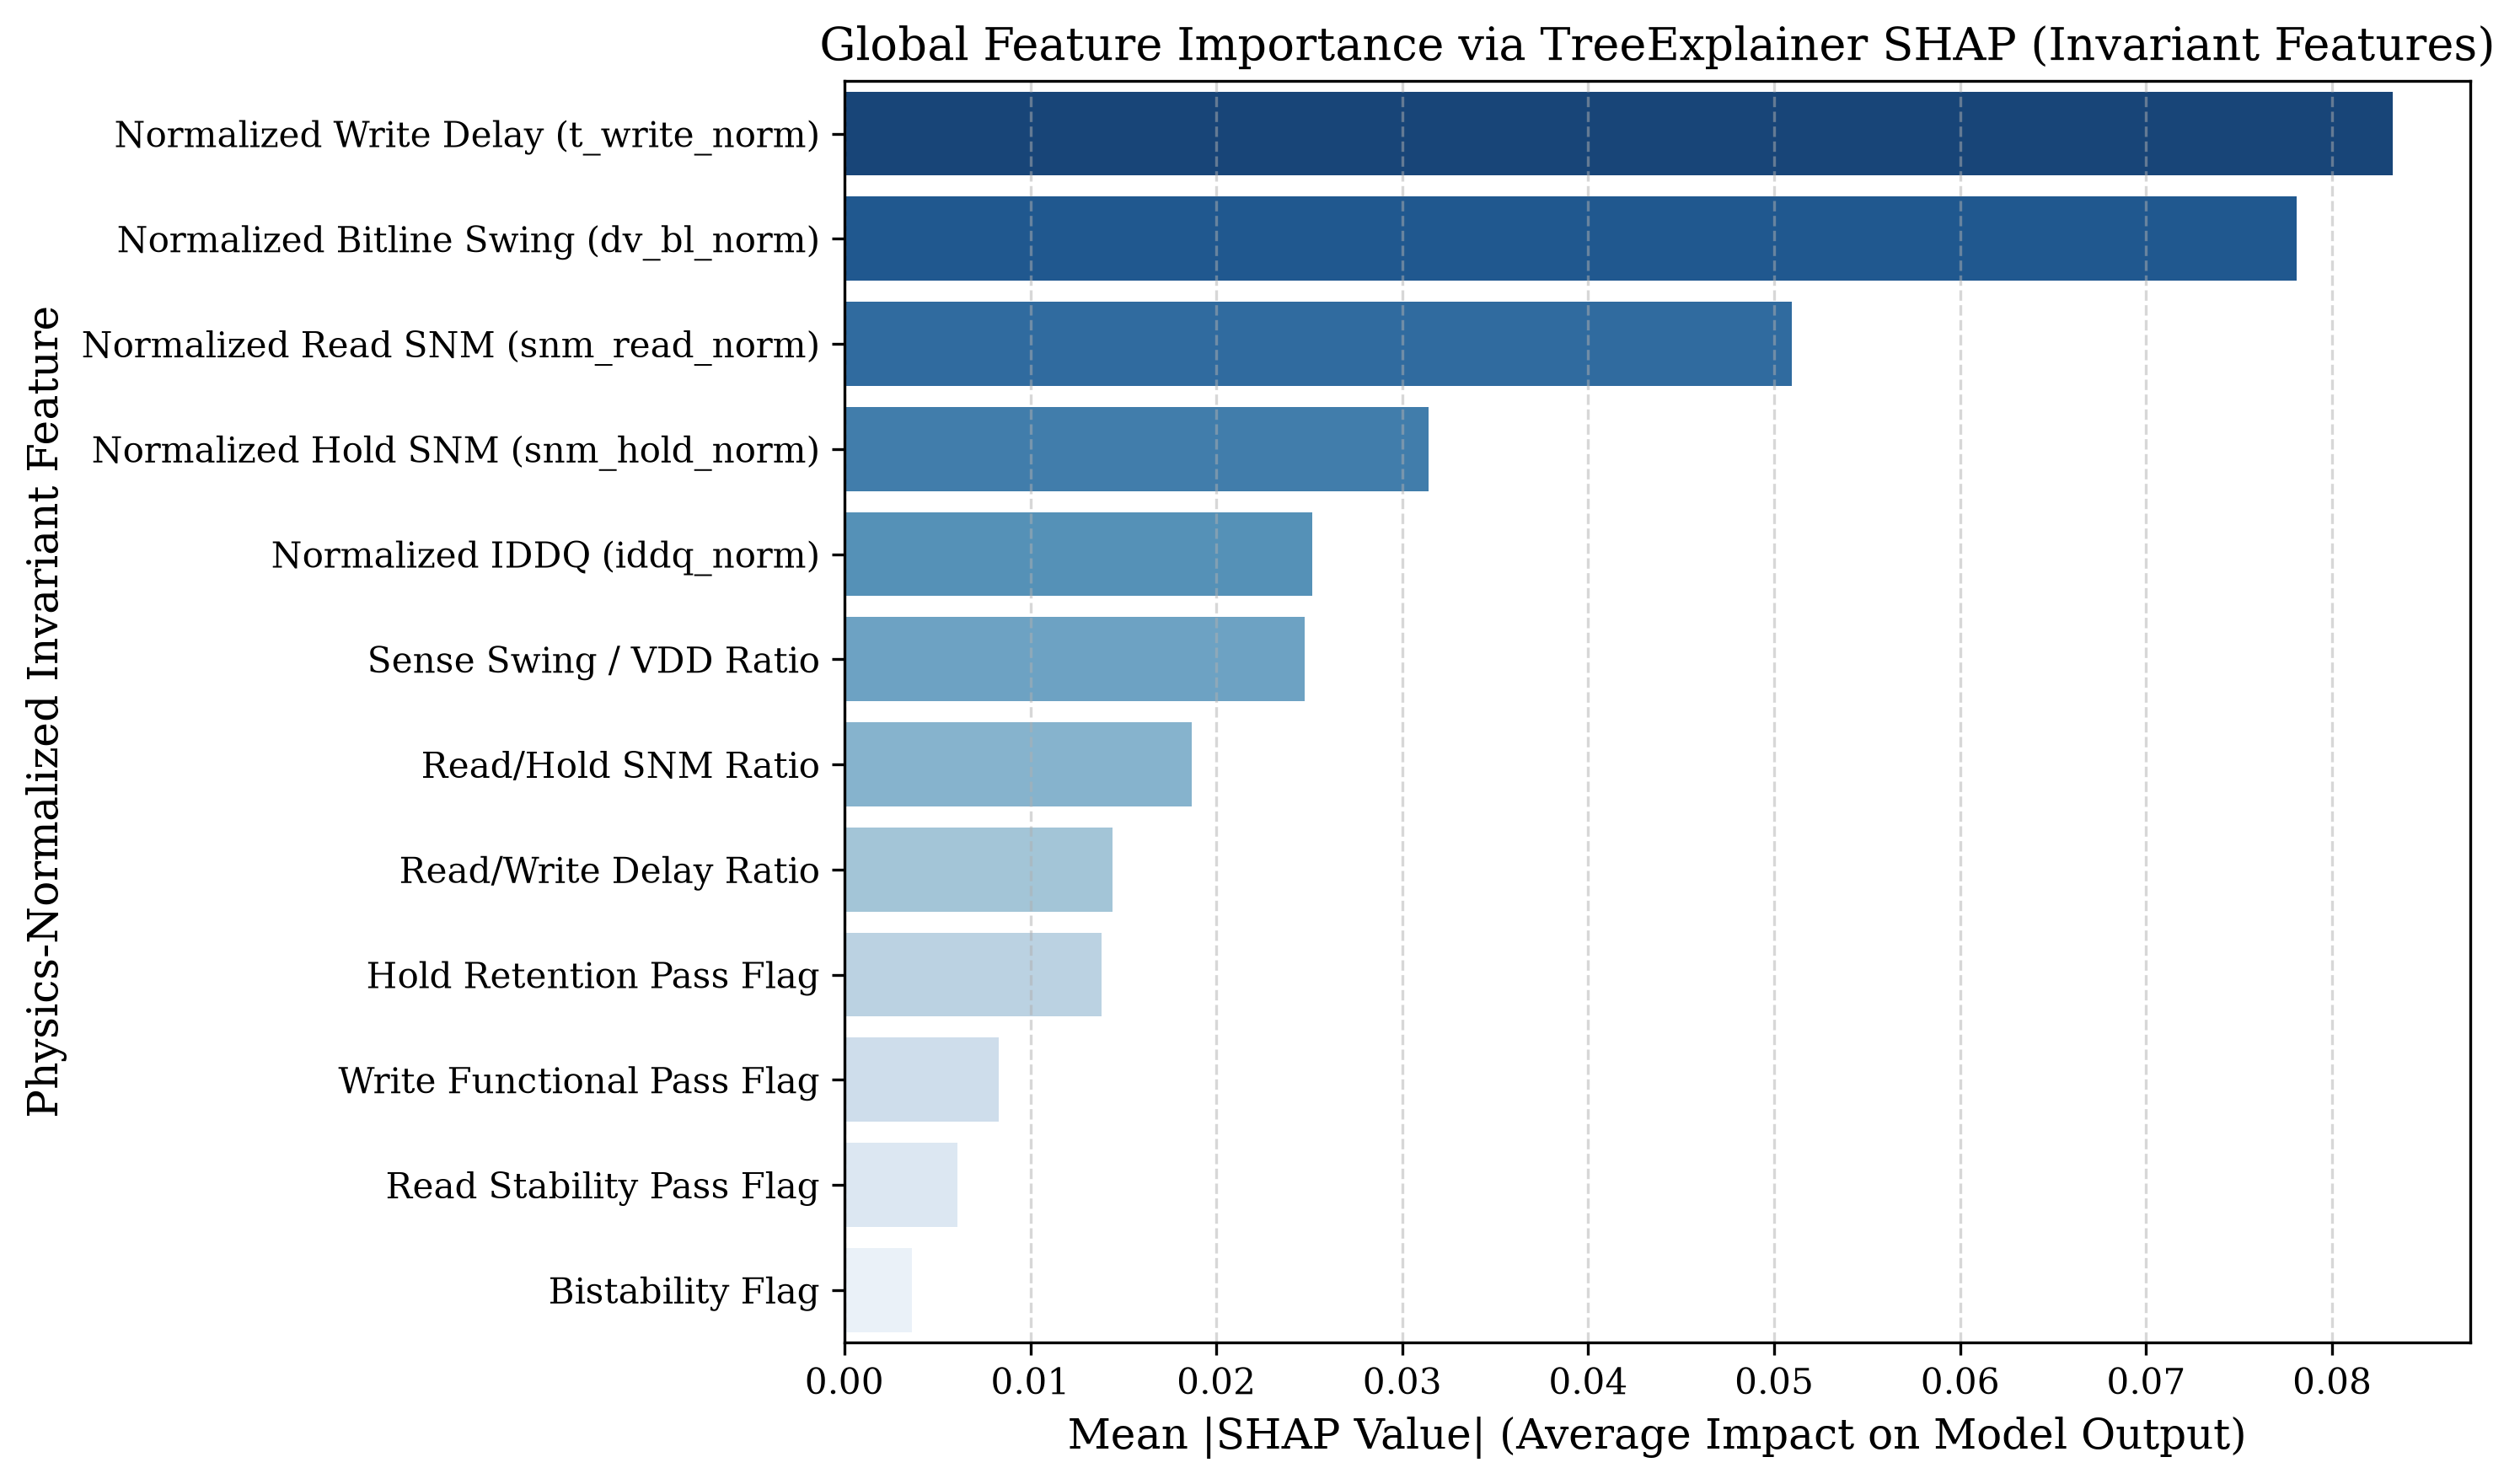
\includegraphics[width=0.98\linewidth]{fig4_shap_summary.png}
\caption{Global feature importance ranking derived from mean absolute SHAP values across the physics-normalized invariant features (450 authentic SPICE samples).}
\label{fig:shap_global}
\end{figure}

\begin{figure}[t]
\centering
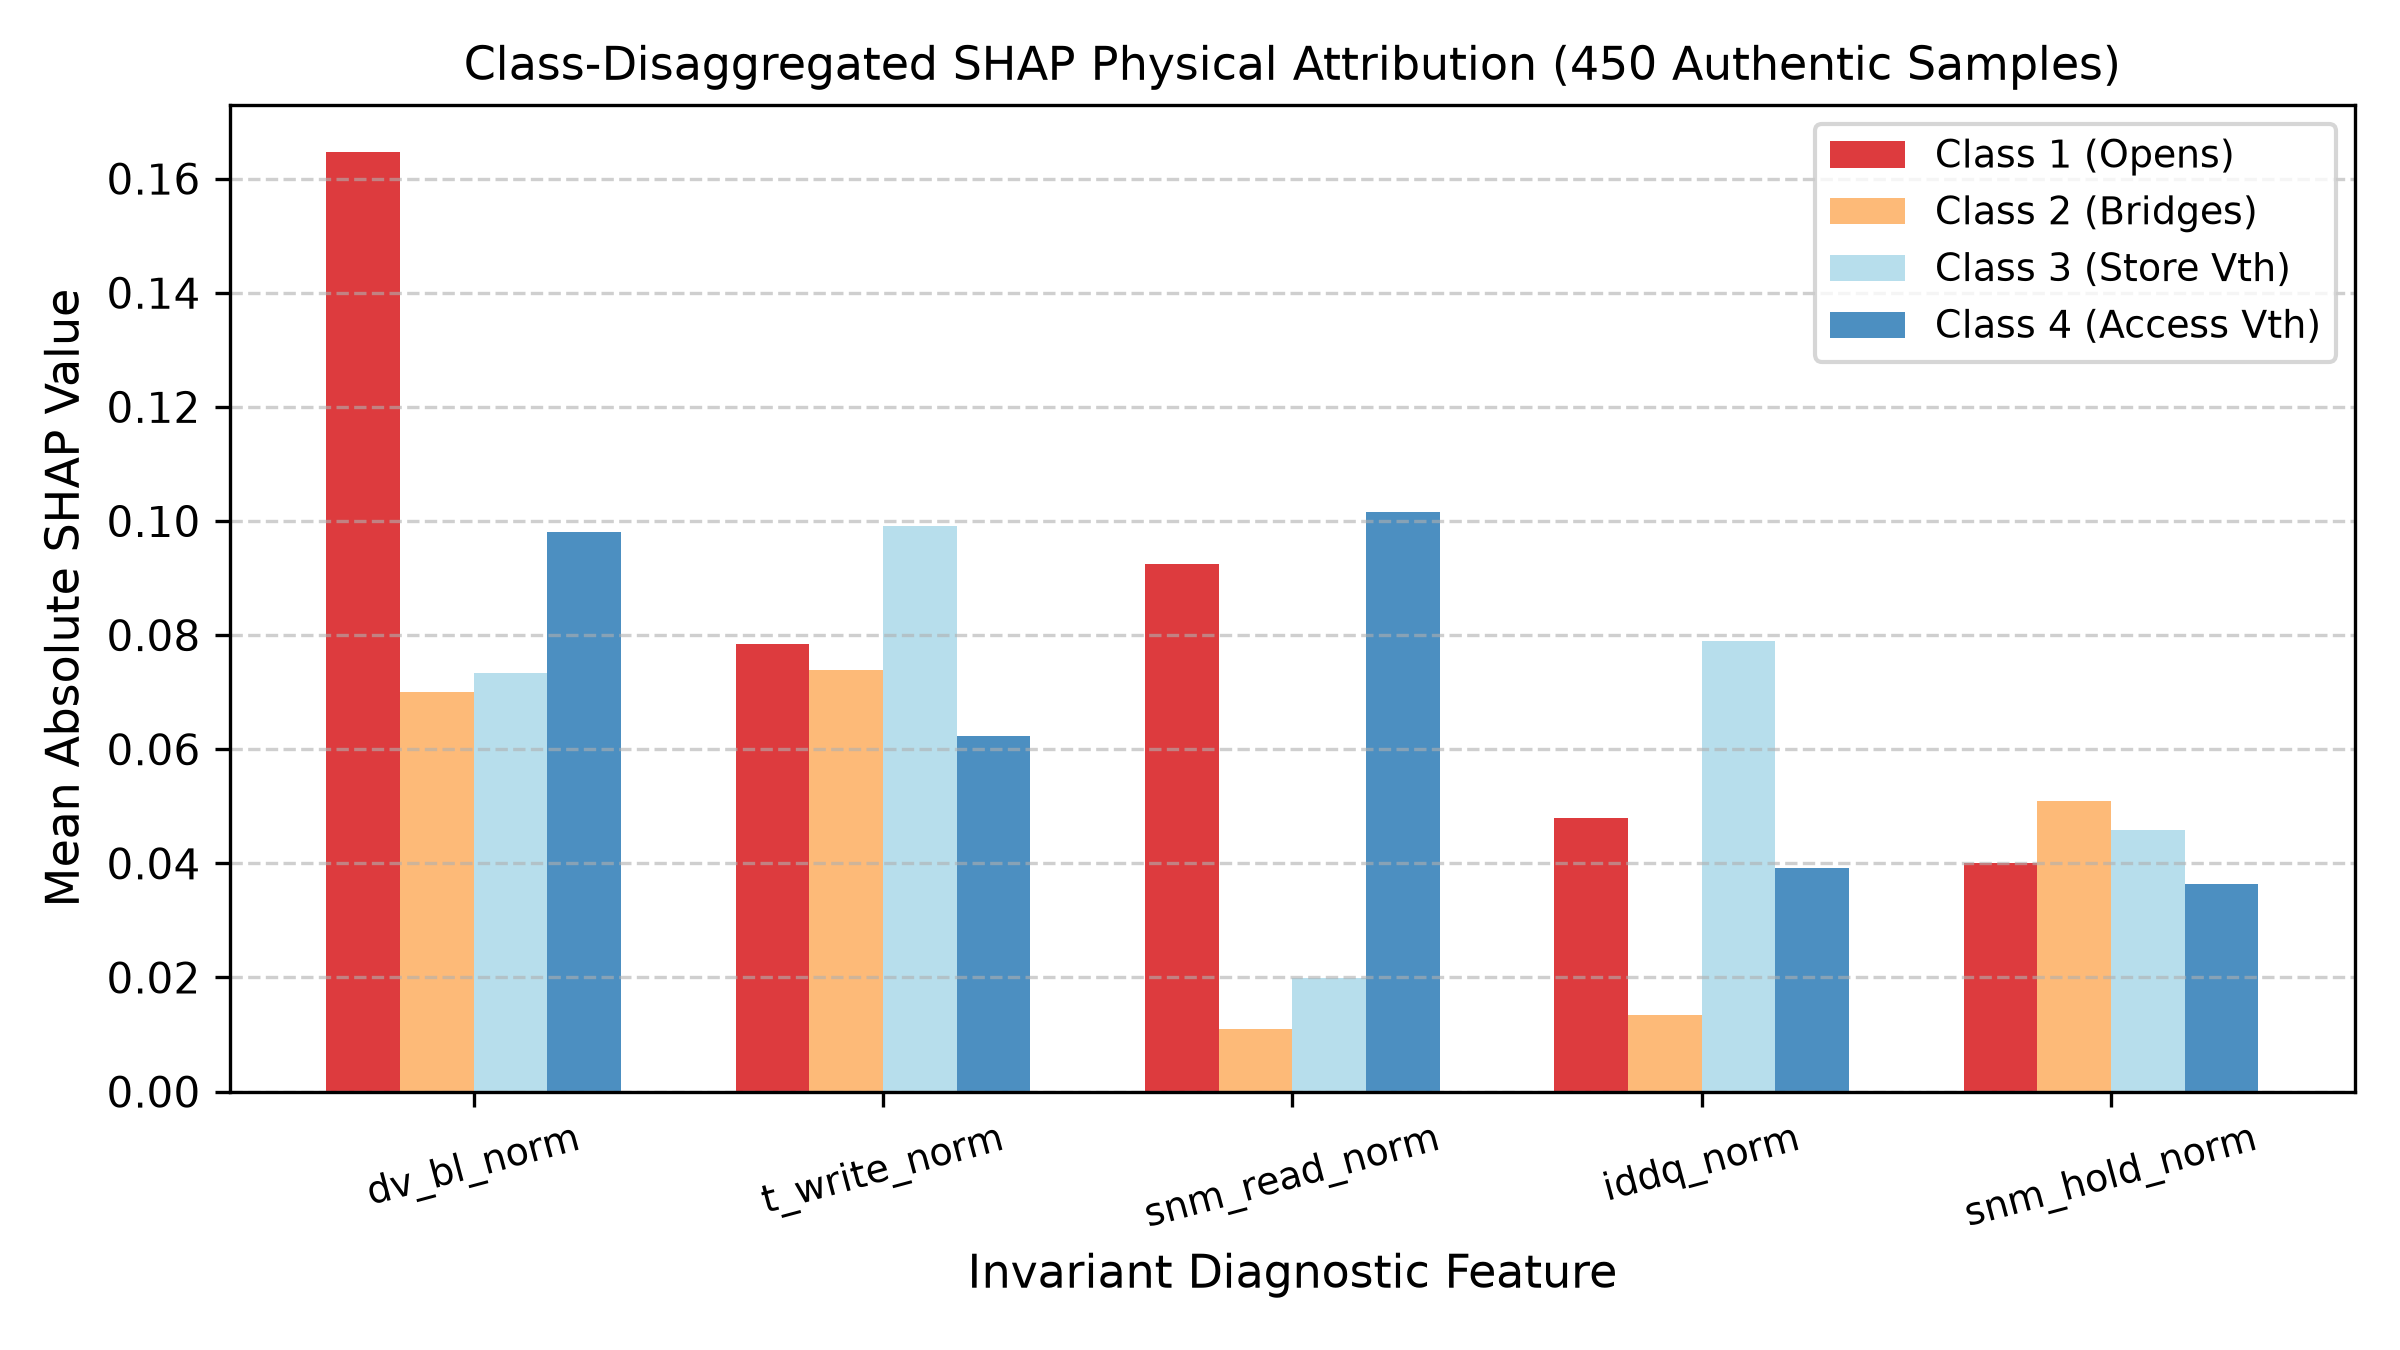
\includegraphics[width=0.98\linewidth]{fig4b_shap_class_importance.png}
\caption{Disaggregated SHAP feature importance by defect class across 450 authentic SPICE samples, demonstrating physical mapping between defect root causes and diagnostic indicators.}
\label{fig:shap_class}
\end{figure}

\subsection{Global Feature Importance Ranking}
As shown in Fig.~\ref{fig:shap_global} and Table~\ref{tab:shap_vals}:
\begin{enumerate}
    \item \textbf{Normalized Bitline Discharge ($\text{dv\_bl\_norm}$, Mean $|SHAP| = 0.0883$):} Serves as the single most critical global diagnostic feature, directly capturing access pass-gate transconductance and read-discharge current drive.
    \item \textbf{Normalized Write Delay ($\text{t\_write\_norm}$, Mean $|SHAP| = 0.0706$):} Second most influential metric, reflecting dynamic state-flip impedance across the cross-coupled inverter pair.
    \item \textbf{Normalized Read SNM ($\text{snm\_read\_norm}$, Mean $|SHAP| = 0.0462$):} Captures cell stability degradation and read-disturb vulnerability during wordline assertion.
    \item \textbf{Normalized Standby Current ($\text{iddq\_norm}$, Mean $|SHAP| = 0.0374$):} Captures quiescent subthreshold leakage anomalies and ohmic bridging shunts.
    \item \textbf{Normalized Hold SNM ($\text{snm\_hold\_norm}$, Mean $|SHAP| = 0.0355$):} Decouples storage inverter degradation from access transistor shifts.
\end{enumerate}

\begin{table}[t]
\centering
\caption{Top Invariant Features Ranked by Mean Absolute SHAP Value (450 Authentic Samples)}
\label{tab:shap_vals}
\resizebox{\columnwidth}{!}{
\begin{tabular}{lccccc}
\toprule
\textbf{Feature Name} & \textbf{Global} & \textbf{Class 1} & \textbf{Class 2} & \textbf{Class 3} & \textbf{Class 4} \\
\midrule
\texttt{dv\_bl\_norm} & \textbf{0.0883} & \textbf{0.1647} & 0.0701 & 0.0734 & \textbf{0.0981} \\
\texttt{t\_write\_norm} & \textbf{0.0706} & 0.0784 & \textbf{0.0739} & \textbf{0.0992} & 0.0624 \\
\texttt{snm\_read\_norm} & 0.0462 & 0.0924 & 0.0109 & 0.0199 & \textbf{0.1016} \\
\texttt{iddq\_norm} & 0.0374 & 0.0480 & 0.0134 & \textbf{0.0790} & 0.0392 \\
\texttt{snm\_hold\_norm} & 0.0355 & 0.0400 & 0.0510 & 0.0459 & 0.0363 \\
\bottomrule
\end{tabular}
}
\end{table}

\subsection{Class-Disaggregated Physical Attribution}
The per-class breakdown illustrated in Fig.~\ref{fig:shap_class} establishes remarkable physical alignment:
\begin{itemize}
    \item \textbf{Class 1 (Resistive Opens):} Heavily driven by \texttt{dv\_bl\_norm} ($0.1647$), \texttt{snm\_read\_norm} ($0.0924$), and \texttt{t\_write\_norm} ($0.0784$). A series resistance at pass-gate $M_5/M_6$ directly throttles the discharge current sinking bitline charge, slowing $\Delta V_{\text{BL}}$ accumulation.
    \item \textbf{Class 2 (Bridging Faults):} Dominated by \texttt{t\_write\_norm} ($0.0739$) and \texttt{dv\_bl\_norm} ($0.0701$). Low-impedance bridging severely collapses bistability, forcing large dynamic write delays.
    \item \textbf{Class 3 ($V_{\text{th}}$ Storage Pair Drift):} Driven by \texttt{t\_write\_norm} ($0.0992$), \texttt{iddq\_norm} ($0.0790$), and \texttt{snm\_hold\_norm} ($0.0459$). Degrading cross-coupled inverter threshold voltages weakens internal latch regeneration and alters subthreshold leakage, while access pass-gate metrics remain unaffected.
    \item \textbf{Class 4 ($V_{\text{th}}$ Access Pair Drift):} Driven by \texttt{snm\_read\_norm} ($0.1016$) and \texttt{dv\_bl\_norm} ($0.0981$), while \texttt{snm\_hold\_norm} is suppressed ($0.0363$). Because access transistors are completely shut off during Hold mode ($WL=0\,\text{V}$), pass-gate threshold drift cannot affect Hold SNM, allowing the model to decouple Class 3 from Class 4 cleanly.
\end{itemize}

% ======================================================================

\section{Stated Limitations}
\label{sec:limits}

To maintain rigorous scientific standards, we note the explicit boundaries of this investigation:
\begin{enumerate}
    \item \textbf{Operational V-T Grid vs. Microscopic Transistor Mismatch:} In this work, operational environmental variation is systematically modeled across 15 Voltage-Temperature operating corners in standard 180\,nm CMOS technology, complemented by empirical reference measurement tolerance studies (Section~\ref{sec:tolerance}). In physical silicon, microscopic intra-die random device mismatch (e.g., Pelgrom-scaled threshold-voltage variations $\sigma(V_{\text{th}}) = A_{V_{\text{th}}} / \sqrt{W \cdot L}$) introduces non-linear stochastic offsets between adjacent transistors; full physical layout-extracted Monte Carlo array characterization represents an important direction for silicon tape-out.
    \item \textbf{Simulation vs Physical Silicon:} All evaluations are conducted using multi-threaded SPICE netlists. While SPICE models provide golden analog precision, physical silicon tape-out introduces unmodeled parasitics, power-grid IR drops, and thermal gradients across large memory arrays.
    \item \textbf{Reference Cell Health and Area Overhead:} The proposed methodology assumes the availability of an on-die healthy reference cell. In practical deployment, reference cell health is established during initial wafer-sort test screening, or via a fault-tolerant triplet of tracking cells with median voting to guard against random local manufacturing defects. In a typical memory macro (e.g., a 1\,Mb array of $1024 \times 1024$ cells), reserving a dedicated tracking cell pair requires $2 / 1{,}048{,}576 \approx 0.00019\%$ of the cell array area. Even in a modular 64\,Kb sub-bank ($256 \times 256$), allocating one tracking cell incurs only $1 / 65{,}536 \approx 0.0015\%$ overhead, well below $0.01\%$.
    \item \textbf{Target Test Architecture:} The extraction of high-resolution analog parameters ($1\,\text{mV}$ DC butterfly sweeps and sub-100ps internal timings) is tailored to post-silicon characterization test vehicles, dedicated scribe-line test structures, and yield-learning macros equipped with analog monitor pass-gates, rather than dense high-volume production array March testing where internal node access is physically constrained.
\end{enumerate}

% ======================================================================

\section{Conclusion}
\label{sec:conclusion}

In this paper, we addressed the critical challenge of cross-environmental diagnostic collapse in machine-learning-based nanoscale SRAM testing. We showed that classical classifiers trained on raw parametric metrics suffer severe out-of-distribution failure when operating across realistic voltage and temperature envelopes, dropping to 46.67\% accuracy. To solve this, we proposed a physics-informed domain adaptation methodology that cancels common-mode environmental shifts using on-die concurrent reference normalization. 

Through an automated SPICE harness executing 3,150 simulation runs across a 15-corner Voltage-Temperature grid (3 supply voltages $\times$ 5 temperatures) in standard 180\,nm CMOS, we validated that invariant feature normalization eliminates environmental dispersion by up to 100.0\% on healthy cells. Under rigorous Leave-One-Corner-Out (LOCO) benchmarking across all 15 corners (450 authentic SPICE samples), the proposed invariant formulation elevated Random Forest and HistGradientBoosting classification accuracy from 70.67\% and 74.00\% to 98.89\% and 98.89\% ($+28.22\%$ and $+24.89\%$ gain), lifting the worst-corner diagnostic floor from 46.67\% to 96.67\% and 93.33\% (with 10 of 15 corners achieving perfect 100.0\% accuracy and exactly 5 total misclassifications across the pooled dataset). Tree SHAP analysis validated that decision boundaries map directly to underlying device physics. This framework suggests feasibility for on-chip or BIST-assisted diagnostic flows in nanoscale SoCs, subject to hardware overhead evaluation.

% ======================================================================

\bibliographystyle{IEEEtran}
\begin{thebibliography}{00}

\bibitem{mukhopadhyay2005modeling}
S.~Mukhopadhyay, H.~Mahmoodi-Meimand, and K.~Roy, ``Modeling and analysis of failure in sub-100-nm ultra-low-power SRAM design,'' \emph{IEEE Trans. Very Large Scale Integr. (VLSI) Syst.}, vol.~13, no.~5, pp.~586--595, May 2005.

\bibitem{marchal2008sram}
P.~Marchal, D.~Appello, P.~Bernardi, M.~Grosso, E.~Sanchez, and M.~Sonza~Reorda, ``SRAM dynamic fault modeling and testing in deep-submicron technologies,'' \emph{IEEE Trans. Very Large Scale Integr. (VLSI) Syst.}, vol.~16, no.~6, pp.~627--640, Jun. 2008.

\bibitem{seevinck1987static}
J.~Seevinck, F.~J.~List, and J.~Lohstroh, ``Static-noise margin analysis of MOS SRAM cells,'' \emph{IEEE J. Solid-State Circuits}, vol.~22, no.~5, pp.~748--754, Oct. 1987.

\bibitem{vandegoor1993march}
A.~J.~van de Goor, ``Using march tests to test SRAMs,'' \emph{IEEE Des. Test Comput.}, vol.~10, no.~1, pp.~8--14, Mar. 1993.

\bibitem{alars2005resistive}
Z.~Al-Ars and A.~J.~van de Goor, ``Impact of resistive opens on SRAM operations and test conditions,'' \emph{IEEE Trans. Comput.-Aided Design Integr. Circuits Syst.}, vol.~24, no.~6, pp.~938--953, Jun. 2005.

\bibitem{pavlov2008sram}
A.~Pavlov and M.~Sachdev, \emph{Defect-Oriented Testing for CMOS SRAMs: Flag-Oriented Test Concepts and Fault Modeling}.\hskip 1em plus 0.5em minus 0.4em\relax Boston, MA: Springer, 2008.

\bibitem{pedregosa2011scikit}
F.~Pedregosa, G.~Varoquaux, A.~Gramfort, V.~Michel, B.~Thirion, O.~Grisel, M.~Blondel, P.~Prettenhofer, R.~Weiss, V.~Dubourg, and J.~Vanderplas, ``Scikit-learn: Machine learning in Python,'' \emph{J. Mach. Learn. Res.}, vol.~12, pp.~2825--2830, Nov. 2011.

\bibitem{lundberg2017unified}
S.~M.~Lundberg and S.-I.~Lee, ``A unified approach to interpreting model predictions,'' in \emph{Proc. Adv. Neural Inf. Process. Syst. (NeurIPS)}, 2017, pp.~4765--4774.

\bibitem{singh2009variability}
A.~Singh, K.~Roy, and V.~De, ``Variability-tolerant SRAM design in sub-45nm CMOS technologies,'' \emph{IEEE Des. Test Comput.}, vol.~26, no.~6, pp.~42--51, Nov. 2009.

\bibitem{stratigopoulos2014ml}
H.-G.~Stratigopoulos, ``Machine learning in analog and mixed-signal test,'' in \emph{Proc. IEEE Eur. Test Symp. (ETS)}, 2014, pp.~1--10.

\bibitem{dasilva2018post}
J.~P.~da Silva, F.~Caldas, and M.~Lubaszewski, ``Machine learning for post-silicon validation and defect diagnosis: A survey,'' \emph{IEEE Trans. Comput.-Aided Design Integr. Circuits Syst.}, vol.~37, no.~11, pp.~2388--2401, Nov. 2018.

\end{thebibliography}

\end{document}
